\section{4th sheaf cobordism}
In this section, we define $cobord_4$, a compactly supported sheaf cobordism between the following squiggly legible diagrams on the support of the cobordism from
\begin{figure}[H]
    \centering
    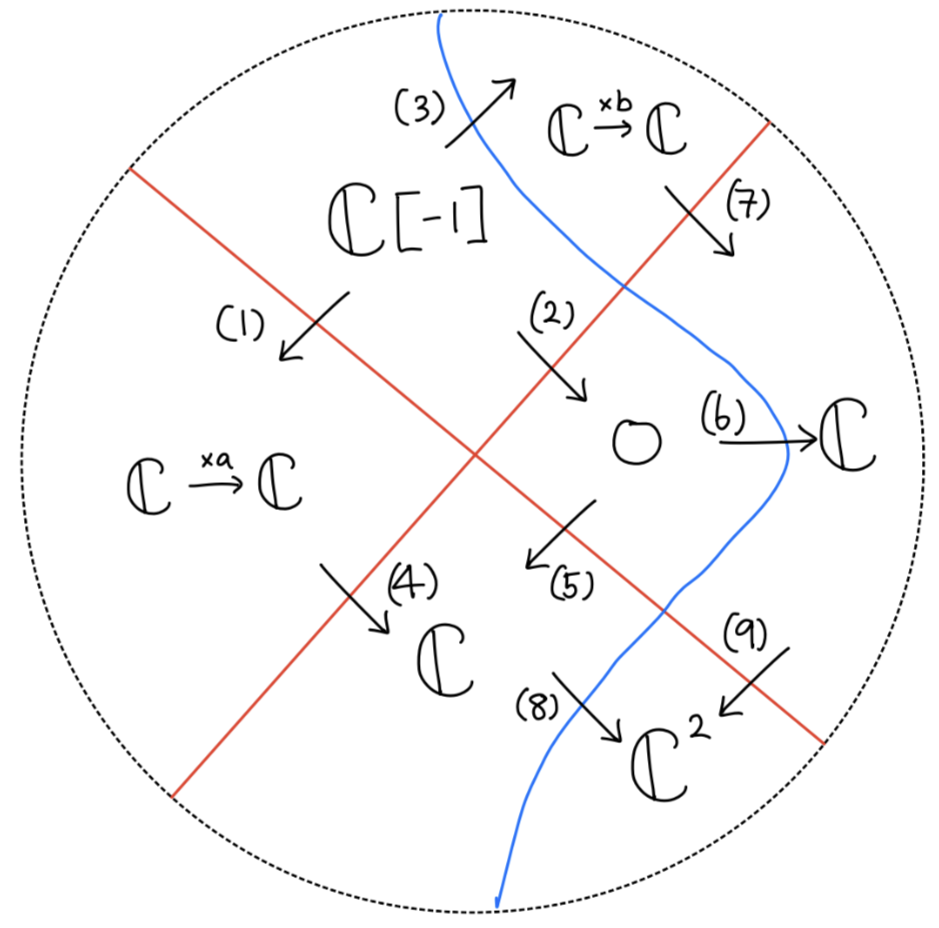
\includegraphics[scale = 0.45]{diagrams/lemma4/21.png}
    \caption{}
    \label{fig:your-label}
\end{figure}
\textbf{Generization maps:}
\begin{enumerate}[label = (\arabic*)]
\item \begin{tikzcd}
\C \arrow[r, "\times 1"]     & \C  \\
0 \arrow[r]\arrow[u] & \C \arrow[u,"\times a"]
\end{tikzcd}

\item \begin{tikzcd}
\C \arrow[r]     & 0  \\
0 \arrow[r]\arrow[u] & 0 \arrow[u]
\end{tikzcd}

\item \begin{tikzcd}
\C \arrow[r, "\times 1"]     & \C  \\
0 \arrow[r]\arrow[u] & \C \arrow[u,"\times b"]
\end{tikzcd}

\item \begin{tikzcd}
\C \arrow[r]     & 0  \\
\C \arrow[r, "\times 1"]\arrow[u,"\times a"] & \C \arrow[u]
\end{tikzcd}

\item \begin{tikzcd}
0 \arrow[r]     & 0  \\
0 \arrow[r]\arrow[u] & \C \arrow[u]
\end{tikzcd}

\item \begin{tikzcd}
0 \arrow[r]     & 0  \\
0 \arrow[r]\arrow[u] & \C \arrow[u]
\end{tikzcd}

\item \begin{tikzcd}
\C \arrow[r]     & 0  \\
\C \arrow[r, "\times 1"]\arrow[u,"\times b"] & \C \arrow[u]
\end{tikzcd}

\item \begin{tikzcd}
0 \arrow[r]     & 0  \\
\C \arrow[r, "\iota_1"]\arrow[u] & \C^2 \arrow[u]
\end{tikzcd}

\item \begin{tikzcd}
0 \arrow[r]     & 0  \\
\C \arrow[r, "\iota_0"]\arrow[u] & \C^2 \arrow[u]
\end{tikzcd}

\end{enumerate}
to
\begin{figure}[H]
    \centering
    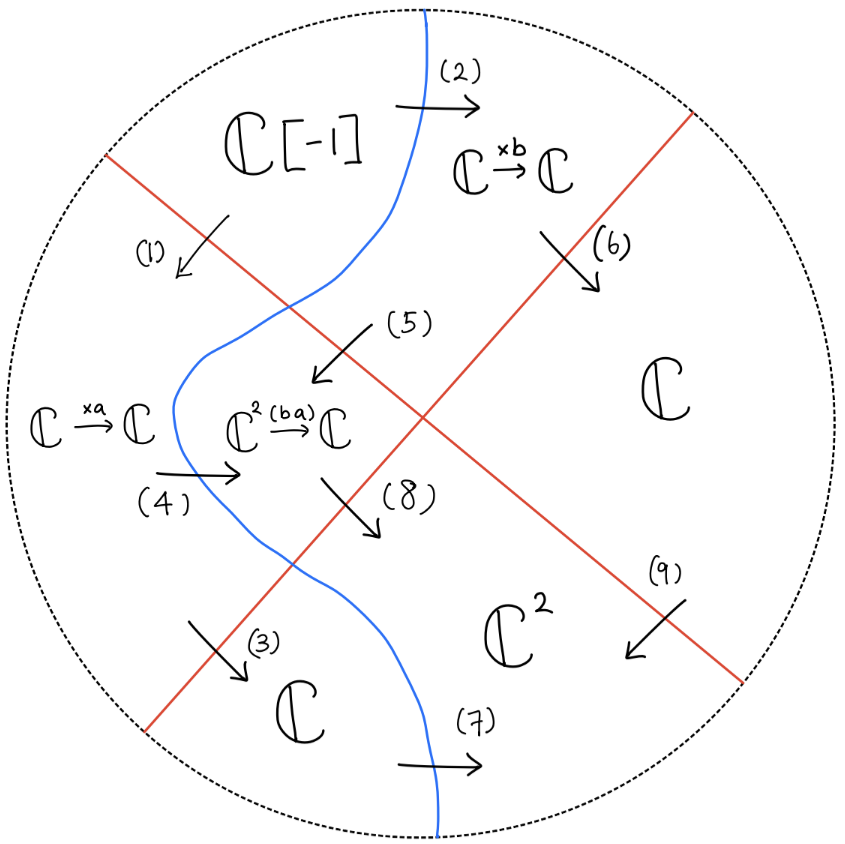
\includegraphics[scale = 0.45]{diagrams/lemma4/33.png}
    \caption{}
    \label{fig:your-label}
\end{figure}
\textbf{Generization maps:}
\begin{enumerate}[label = (\arabic*)]
\item \begin{tikzcd}
\C \arrow[r, "\times 1"]     & \C  \\
0 \arrow[r]\arrow[u] & \C \arrow[u,"\times a"]
\end{tikzcd}

\item \begin{tikzcd}
\C \arrow[r, "\times 1"]     & \C  \\
0 \arrow[r]\arrow[u] & \C \arrow[u,"\times b"]
\end{tikzcd}

\item \begin{tikzcd}
\C \arrow[r]     & 0  \\
\C \arrow[r, "\times 1"]\arrow[u,"\times a"] & \C \arrow[u]
\end{tikzcd}

\item \begin{tikzcd}
\C \arrow[r, "\times 1"]     & \C  \\
\C \arrow[r, "\iota_1"]\arrow[u,"\times a"] & \C^2 \arrow[u, "(b ~ a)"]
\end{tikzcd}

\item \begin{tikzcd}
\C \arrow[r, "\times 1"]     & \C  \\
\C \arrow[r, "\iota_0"]\arrow[u,"\times b"] & \C^2 \arrow[u, "(b ~ a)"]
\end{tikzcd}

\item \begin{tikzcd}
\C \arrow[r]     & 0  \\
\C \arrow[r, "\times 1"]\arrow[u,"\times b"] & \C \arrow[u]
\end{tikzcd}

\item \begin{tikzcd}
0 \arrow[r]     & 0  \\
\C \arrow[r, "\iota_1"]\arrow[u] & \C^2 \arrow[u]
\end{tikzcd}

\item \begin{tikzcd}
\C \arrow[r]     & 0  \\
\C^2 \arrow[r, "id"]\arrow[u,"(b~a)"] & \C^2 \arrow[u]
\end{tikzcd}

\item \begin{tikzcd}
0 \arrow[r]     & 0  \\
\C \arrow[r, "\iota_0"]\arrow[u] & \C^2 \arrow[u]
\end{tikzcd}

\end{enumerate}

\subsection*{Notations}
%definition of a Riemann sphere with two punctures
\begin{definition}
$M$ denotes a Riemann sphere with two punctures at $0$ and $\infty$. $M$ is diffeomorphic to a cylinder.
\end{definition}
%definition of \Phi_t^{symbol}, \Xi_t^{symbol}
\begin{definition}
For $t_0\in\{0,1\}$ and $symbol\in\{0,\infty, squig \}$
\begin{enumerate}
\item we denote $\Phi_{t_0}^{symbol}$ to be smooth maps
\begin{align*}
&\Phi_{t_0}^0 : (S^1)^n \rightarrow M \\
&\Phi_{t_0}^\infty : (S^1)^m \rightarrow M \\
&\Phi_{t_0}^{squig} : [0,1]^{k_{t_0}} \rightarrow M
\end{align*}

\item we denote $\Xi_{t_0}^{symbol}$ a co-orientation of $\Phi_{t_0}^{symbol}$.

\item we denote the pair $(\Phi_{t_0}^{symbol},\Xi_{t_0}^{symbol})$ as $\Lambda_{t_0}^{symbol}$. When $symbol \in \{0,\infty\}$, this could be thought as a front projection of a Legendrian living inside the cocircle bundle of $M$, so we will use $\Lambda_{t_0}^{symbol}$ to denote both

\item we denote the triple $(\Lambda_{t_0}^{0},\Lambda_{t_0}^{\infty},\Lambda_{t_0}^{squig})$ as $\Lambda_{t_0}$ and call it the squiggly diagram at $t_0$. Later in the section, $\Lambda_0$ will be used to denote the squiggly diagram at the beginning of the isotopy underlying $cobord_4$ and $\Lambda_1$ will be used to denote the squiggly diagram at the end of the isotopy underlying $cobord_4$. 
\end{enumerate}
\end{definition}

%definition of \Phi_\bullet^{symbol}, \Xi_\bullet^{symbol}
\begin{definition}
For $symbol\in\{0,\infty, squig \}$
\begin{enumerate}
\item we denote $\Phi_\bullet^{symbol}$ to be smooth maps
\begin{align*}
&\Phi_\bullet^0 : (S^1)^n \times [0,1]_t \rightarrow M \times [0,1]_t \\
&\Phi_\bullet^\infty : (S^1)^m \times [0,1]_t \rightarrow M \times [0,1]_t \\
&\Phi_\bullet^{squig} : \coprod_{1\leq i \leq k} ([0,1] \times [a_i,b_i]_t) \rightarrow M \times [0,1]_t
\end{align*}
where the maps are identity maps on the time coordinates. I added auxiliary subscript `$t$' to distinguish the time coordinates from the space coordinates.

\item we denote $\Xi_\bullet^{symbol}$ a co-orientation of $\Phi_\bullet^{symbol}$.

\item we denote the pair $(\Phi_\bullet^{symbol},\Xi_\bullet^{symbol})$ as $\Lambda_\bullet^{symbol}$. Later in the section, $\Lambda_\bullet^{symbol}$ will be used to denote the an isotopy from $\Lambda_0^{symbol}$ to $\Lambda_1^{symbol}$ underlying $cobord_4$.

\item we denote the triple $(\Lambda_\bullet^{0},\Lambda_\bullet^{\infty},\Lambda_\bullet^{squig})$ as $\Lambda_\bullet$ and call it a squiggly isotopy from $\Lambda_0$ to $\Lambda_1$. Later in the section, $\Lambda_\bullet$ will be used to denote the isotopy between squiggly diagrams starting from $\Lambda_0$ ending at $\Lambda_1$ underlying $cobord_4$.
\end{enumerate}
\end{definition}

%definition of a bump function
\begin{definition}
For $t \in [0,1]$, we define $\Psi_t: \R \rightarrow \R$ to be a bump function parametrized by $t$ as follows
\[\Psi_t(x)=\bigg\{
\begin{array}{ll}
    e^{(\frac{x^2}{x^2 - 1})}(\frac{1}{2}-t) & \text{if } |x| < 1 \\
    0 & \text{if } |x| \geq 1
\end{array}
\bigg.
\]
Note that 
\begin{itemize}
\item $supp(\Psi_t) = [-1,1]$ if $t\neq \frac{1}{2}$

\item $\{(1,0)$, $(-1,0),(0, \frac{1}{2}-t)\} \subset Graph(\Psi_t)$
\end{itemize}
\end{definition}

%definition of standard disks
\begin{definition}
We denote the standard open disk in $\R^2$ of radius $r_0$ centered at the origin as 
\[
D_{r=r_0} := \{(x,z)\rightarrow \R^2 ~|~ x^2+z^2 < r_0^2\}
\]
For $t_0 \in [0,1]$, we canonically identify $D_{r=r_0}\times \{t_0\}$ with $D_{r=r_0}$ using the following diffeomorphism
\begin{align*}
& D_{r=r_0} \xrightarrow{\sim} D_{r=r_0} \times \{t_0\} \\
& (x,z) \mapsto (x,z,t_0)
\end{align*}
and with abuse of expression say that sheaves on $D_{r=r_0}\times \{t_0\}$ as sheaves on $D_{r=r_0}$.
\end{definition}

%definition of subsets of D_{r=2}\times \{0\} and their co-orientations
\begin{definition}
\begin{enumerate}
\item We define the following subsets of $D_{r=2} \cong D_{r=2}\times \{0\}$
\begin{itemize}
\item $\lambda_0^0 := \{(x,z) \in D_{r=2} ~|~ x = \Psi_0(z)\}$

\item $\lambda_0^\infty$ is the union of the following two components
\begin{enumerate}[label=(\roman*)]
\item $\{(x,z) \in D_{r=2} ~|~ z = x \}$

\item $\{(x,z) \in D_{r=2} ~|~ z = -x \}$
\end{enumerate}
\end{itemize}

\item We define co-orientations $\xi_0^{symbol}$ of $\lambda_0^{symbol}$ as follows
\begin{itemize}
\item $\xi_0^0$: hairs are pointing towards the left i.e. coefficients of $dx$ are negative.

\item $\xi_0^\infty$: hairs are pointing towards the left i.e. coefficients of $dx$ are positive.
\end{itemize}
\end{enumerate}
\end{definition}

%definition of subsets of D_{r=2}\times \{1\} and their co-orientations
\begin{definition}
\begin{enumerate}
\item We define the following subsets of $D_{r=2} \cong D_{r=2}\times \{1\}$
\begin{itemize}
\item $\lambda_1^0 := \{(x,z) \in D_{r=2} ~|~ x = \Psi_1(z)\}$

\item $\lambda_1^\infty$ is the union of the following two components
\begin{enumerate}[label=(\roman*)]
\item $\{(x,z) \in D_{r=2} ~|~ z = x \}$

\item $\{(x,z) \in D_{r=2} ~|~ z = -x \}$
\end{enumerate}
\end{itemize}

\item We define co-orientations $\xi_1^{symbol}$ of $\lambda_1^{symbol}$ as follows
\begin{itemize}
\item $\xi_1^0$: hairs are pointing towards the left i.e. coefficients of $dx$ are negative.

\item $\xi_1^\infty$: hairs are pointing upward direction i.e. coefficients of $dz$ are positive.
\end{itemize}
\end{enumerate}
\end{definition}

%definition of subsets of D_{r=2}\times [0,1] and their co-orientations
\begin{definition}
\begin{enumerate}
\item We define the following subsets of $D_{r=2}\times [0,1]$
\begin{itemize}
\item $\lambda_\bullet^0 := \{(x,z,t) \in D_{r=2} \times [0,1] ~|~ x = \Psi_t(z)\}$

\item $\lambda_\bullet^\infty$ is the union of the following two components
\begin{enumerate}[label=(\roman*)]
\item $\{(x,z,t) \in D_{r=2}\times [0,1] ~|~ z = x \}$

\item $\{(x,z,t) \in D_{r=2}\times [0,1] ~|~ z = -x \}$
\end{enumerate}
\end{itemize}

\item We define co-orientations $\xi_\bullet^{symbol}$ of $\lambda_\bullet^{symbol}$ as follows
\begin{itemize}
\item $\xi_\bullet^0$: hairs are pointing towards the left i.e. coefficients of $dx$ are negative.

\item $\xi_\bullet^\infty$: hairs are pointing upward direction i.e. coefficients of $dz$ are positive.
\end{itemize}
\end{enumerate}
\end{definition}

% stratifications \mathcal{S}_??
\begin{definition}
\begin{enumerate}
\item Consider a stratification $\mathcal{S}_0$ on $D_{r=2}$ induced by $\lambda_0$ i.e. stratification where $0$ dimensional strata are either crossings or end points of squiggly lines, $1$ dimensional strata are sub-arcs of co-oriented links and squiggly lines that are separated by $0$ dimensional strata, and $2$ dimensional strata are exactly the connected components of $M-\lambda_0$. Note that $1$ dimensional strata has co-orientations inherited from $\lambda_0$.

\item Consider a stratification $\mathcal{S}_1$ on $D_{r=2}$ induced by $\lambda_1$ i.e. stratification where $0$ dimensional strata are either crossings or end points of squiggly lines, $1$ dimensional strata are sub-arcs of co-oriented links and squiggly lines that are separated by $0$ dimensional strata, and $2$ dimensional strata are exactly the connected components of $M-\lambda_1$. Note that $1$ dimensional strata has co-orientations inherited from $\lambda_1$.
\end{enumerate}

\item Consider a stratification $\mathcal{S}_\bullet$ on $D_{r=2}\times [0,1]$ induced by $\lambda_\bullet$ i.e. strata are non-empty finite intersections of $\lambda_\bullet^0$, $\lambda_\bullet^\infty$, and $\lambda_\bullet^{squig}$. Note that $2$ dimensional strata has co-orientations inherited from $\lambda_\bullet$.
\end{definition}

Now let's list the strata of $\mathcal{S}_0$, $\mathcal{S}_1$, and $\mathcal{S}_\bullet$ using the following notations:
%definition of sgn function
\begin{definition}
$\operatorname{sgn} : \R \rightarrow \{-,0,+ \}$ is defined as 
\[\operatorname{sgn}(x)=\left\{
\begin{array}{ll}
    + & \text{if } x > 0 \\
    0 & \text{if } x = 0 \\
	- & \text{if } x < 0 \\
\end{array}
\right.
\]
\end{definition}

% +,0,- notations of strata s_{t_0}
\begin{definition}
For $i = 1,2,3$ , $t_0 = 0,1$, and $sgn_i \in \{-,0,+\}$, we define
\begin{align*}
s_{t_0}(sgn_1,sgn_2,sgn_3):=~ &\{(x,z) \in D_{r=2}\cong D_{r=2}\times \{t_0\} ~| \\
&\operatorname{sgn}(x-\Psi_{t_0}(z))=sgn_1,~ \operatorname{sgn}(x-z)=sgn_2,\\ 
&\operatorname{sgn}((-x-z)=sgn_3\}
\end{align*}
\end{definition}

% +,0,- notations of strata s_\bullet
\begin{definition}
For $i = 1,2,3$ and $sgn_i \in \{-,0,+\}$, we define
\begin{align*}
s_\bullet(sgn_1,sgn_2,sgn_3):=~ &\{(x,z,t) \in D_{r=2}\times [0,1] ~| \\
&\operatorname{sgn}(x-\Psi_{t}(z))=sgn_1,~ \operatorname{sgn}(x-z)=sgn_2,\\ 
&\operatorname{sgn}((-x-z)=sgn_3\}
\end{align*}
\end{definition}


\begin{definition}
Now I will describe $\mathcal{S}_0$, $\mathcal{S}_1$, and $\mathcal{S}_\bullet$ using the above notations:
\begin{enumerate}
\item $\mathcal{S}_0$:
\begin{itemize}
\begin{figure}[H]
    \centering
    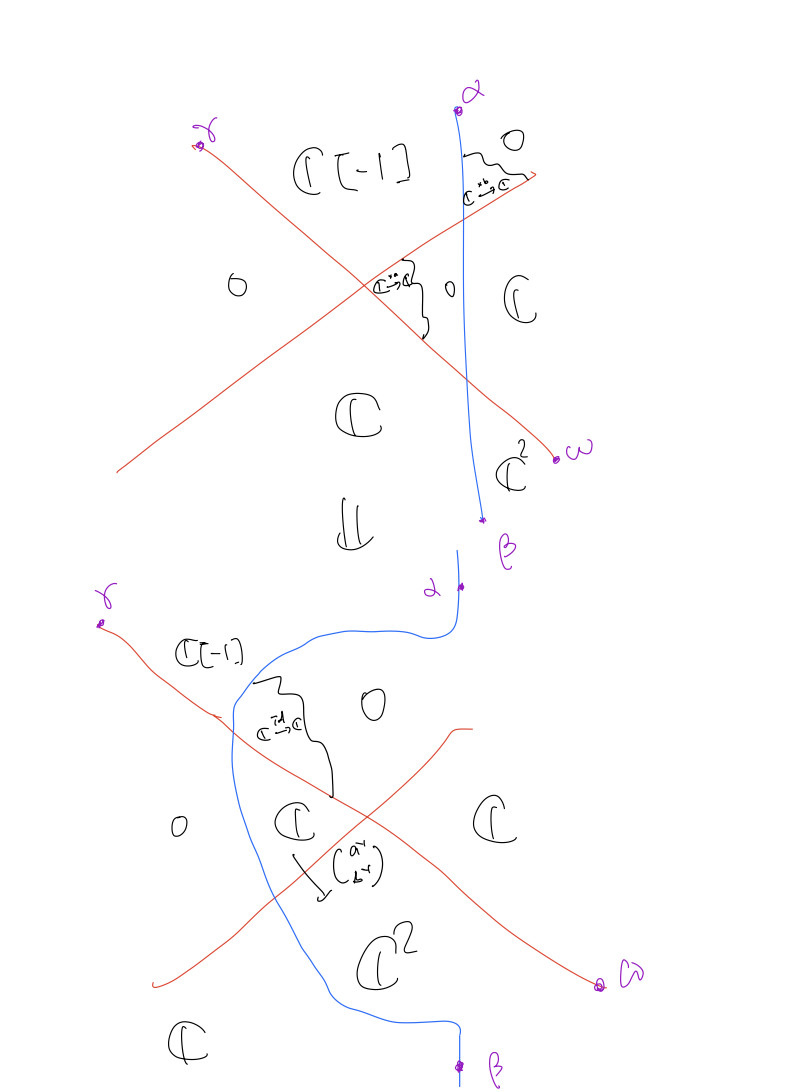
\includegraphics[scale = 0.45]{diagrams/lemma4/1.png} 
    \caption{}
    \label{fig:your-label}
\end{figure}
\item $2$ dimensional strata: \\
$\{s_0(sgn_2,sgn_1,sgn_3) ~|~ sgn_i \in \{-,+\}\text{ for i=1,2,3, except } s_0(+,-,+)\}$

\begin{figure}[H]
    \centering
    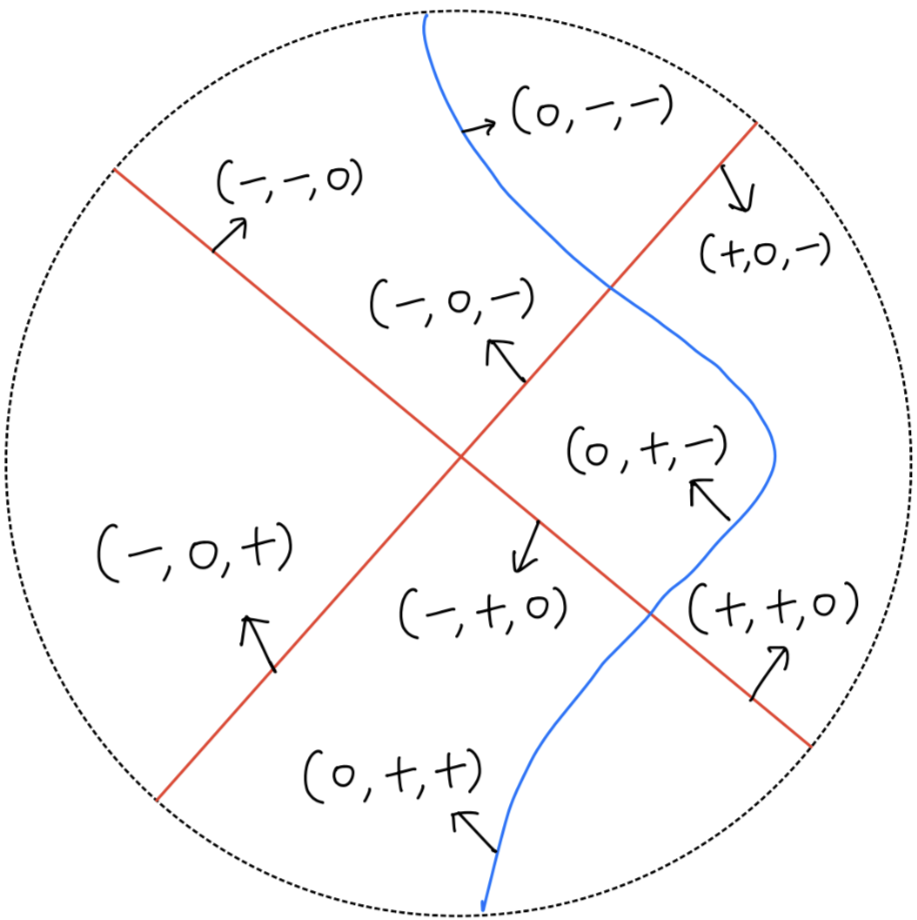
\includegraphics[scale = 0.45]{diagrams/lemma4/2.png}
    \caption{}
    \label{fig:your-label}
\end{figure}
\item $1$ dimensional strata:\\
$\{s_0(0,sgn_2,sgn_3) ~|~ sgn_i \in \{-,+\}\text{ for i=2,3, except } s_0(0,-,+)\}\\
\cup\{s_0(sgn_1,0,sgn_3) ~|~ sgn_i \in \{-,+\}\text{ for i=1,3, except } s_0(+,0,+)\}\\
\cup\{s_0(sgn_1,sgn_2,0) ~|~ sgn_i \in \{-,+\}\text{ for i=1,2, except } s_0(+,-,0)\}$ 

\begin{figure}[H]
    \centering
    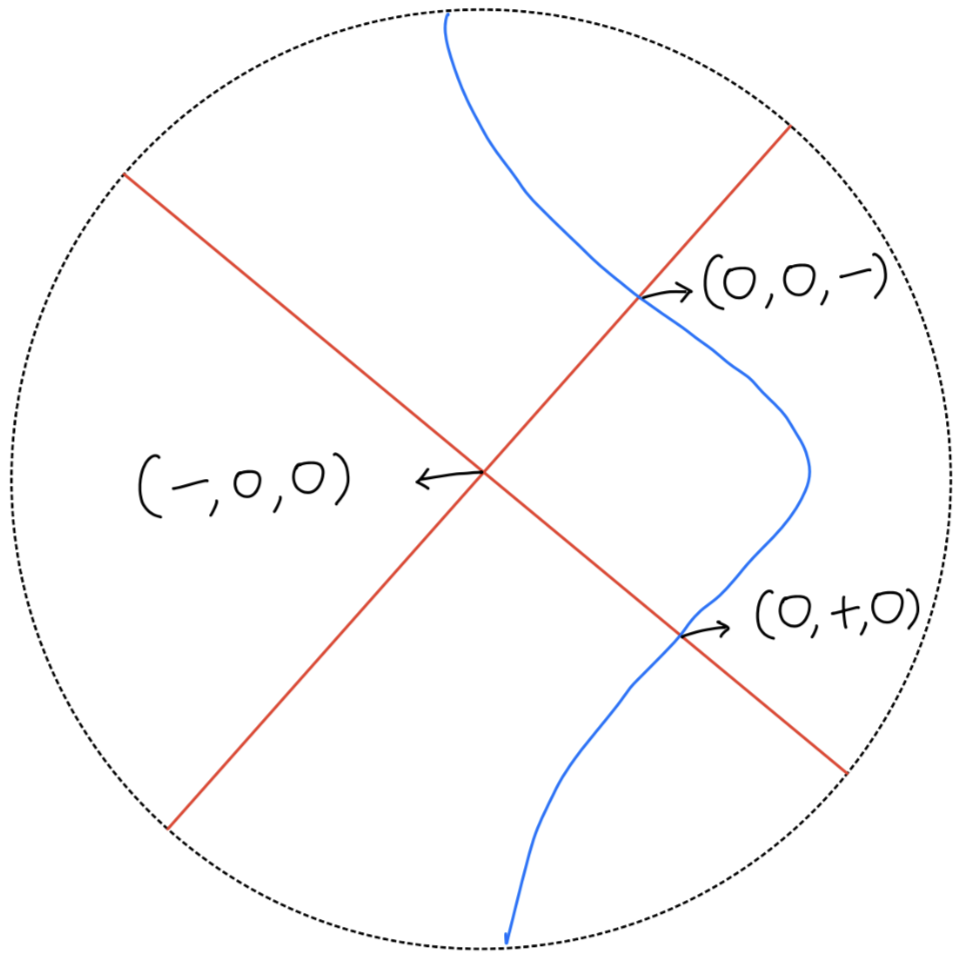
\includegraphics[scale = 0.45]{diagrams/lemma4/3.png}
    \caption{}
    \label{fig:your-label}
\end{figure}
\item $0$ dimensional strata: \\
$s_0(-,0,0)$, $s_0(0,0,-)$, $s_0(0,+,0)$
\end{itemize}

\item $\mathcal{S}_1$:
\begin{itemize}
\begin{figure}[H]
    \centering
    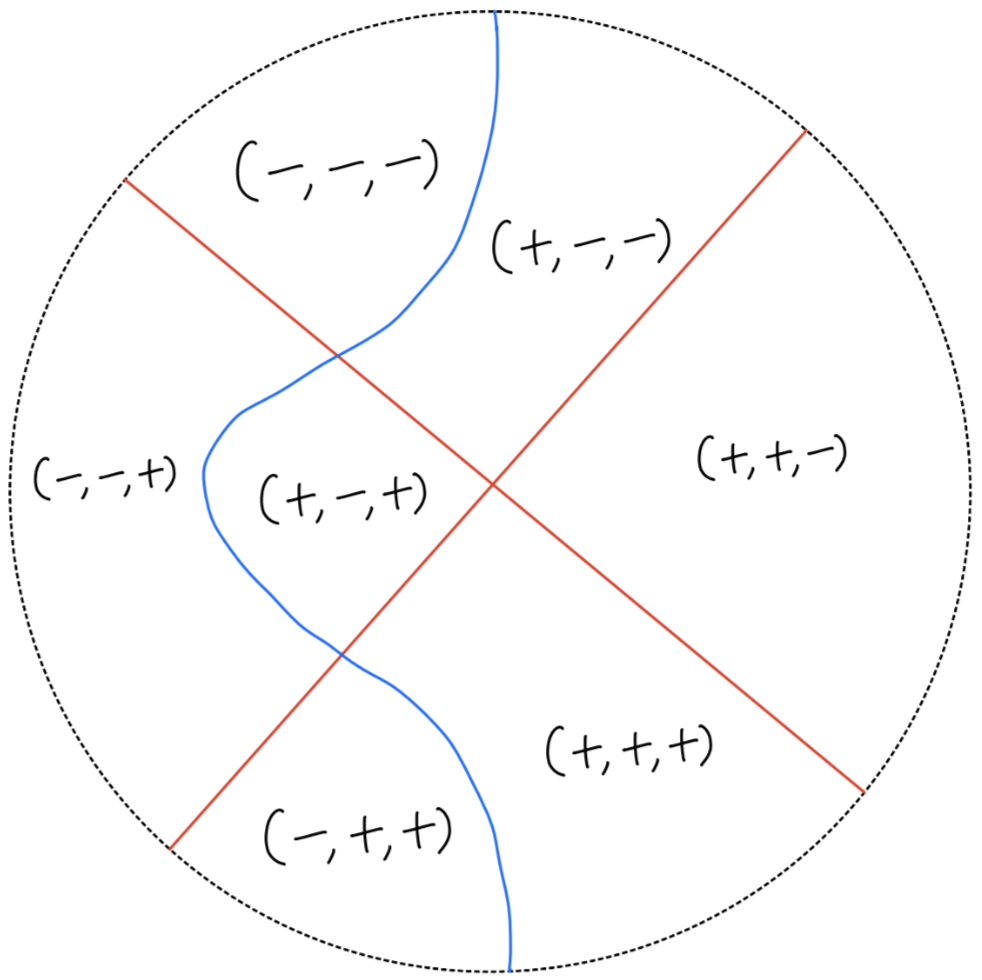
\includegraphics[scale = 0.45]{diagrams/lemma4/4.png}
    \caption{}
    \label{fig:your-label}
\end{figure}
\item $2$ dimensional strata: \\
$\{s_1(sgn_2,sgn_1,sgn_3) ~|~ sgn_i \in \{-,+\}\text{ for i=1,2,3, except } s_1(-,+,-)\}$

\begin{figure}[H]
    \centering
    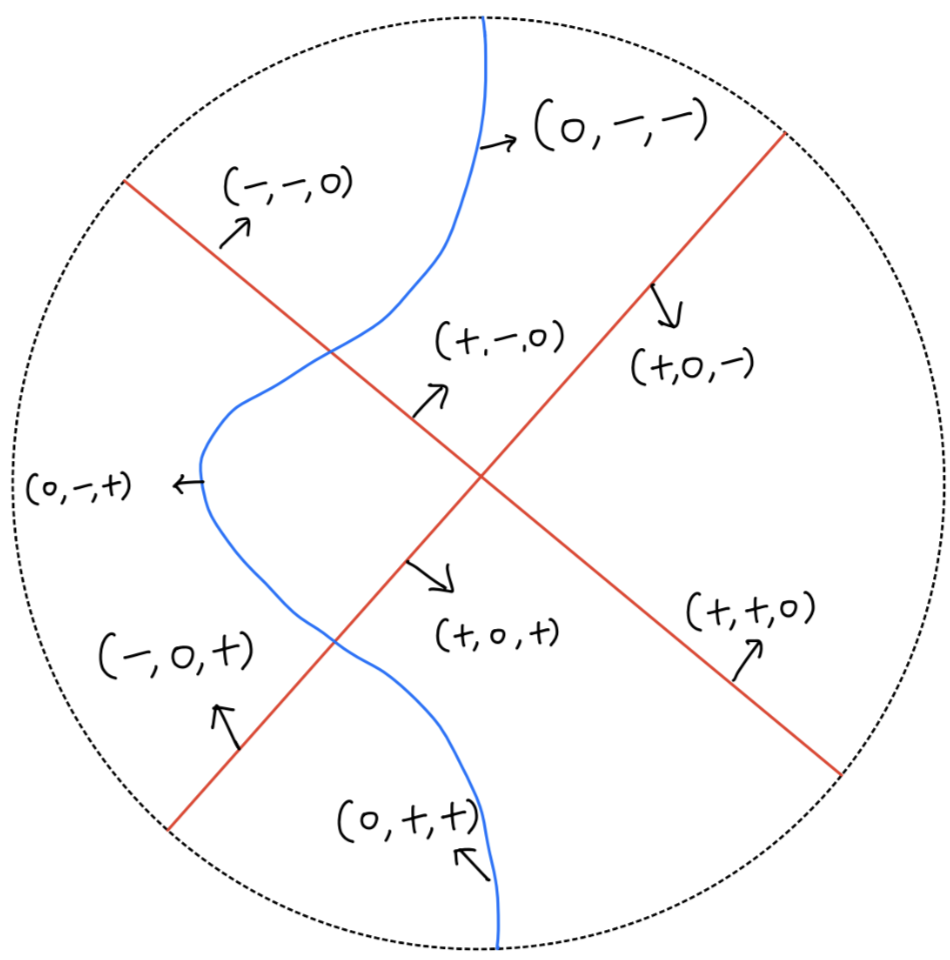
\includegraphics[scale = 0.45]{diagrams/lemma4/5.png}
    \caption{}
    \label{fig:your-label}
\end{figure}
\item $1$ dimensional strata:\\
$\{s_1(0,sgn_2,sgn_3) ~|~ sgn_i \in \{-,+\}\text{ for i=2,3, except } s_1(0,+,-)\}\\
\cup\{s_1(sgn_1,0,sgn_3) ~|~ sgn_i \in \{-,+\}\text{ for i=1,3, except } s_1(-,0,-)\}\\
\cup\{s_1(sgn_1,sgn_2,0) ~|~ sgn_i \in \{-,+\}\text{ for i=1,2, except } s_1(-,+,0)\}$ 

\begin{figure}[H]
    \centering
    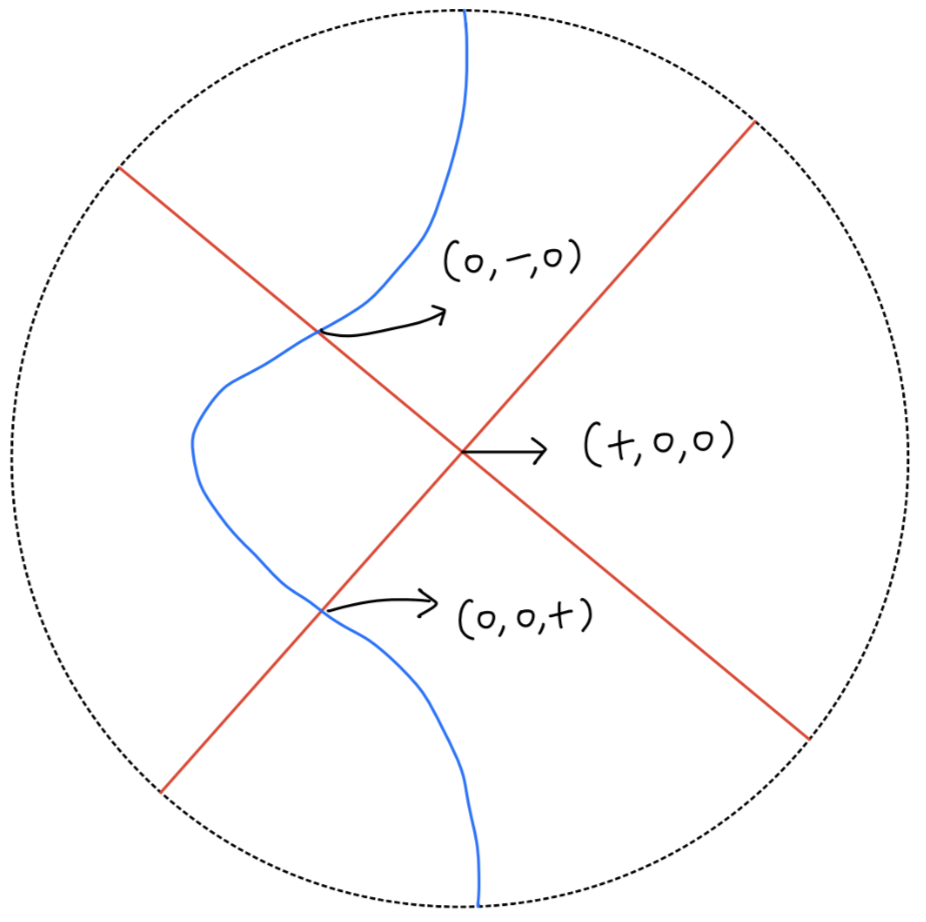
\includegraphics[scale = 0.45]{diagrams/lemma4/6.png}
    \caption{}
    \label{fig:your-label}
\end{figure}
\item $0$ dimensional strata: \\
$s_1(0,-,0)$, $s_1(+,0,0)$, $s_1(0,0,+)$
\end{itemize}

\item $\mathcal{S}_\bullet$:
\begin{itemize}
\begin{figure}[H]
    \centering
    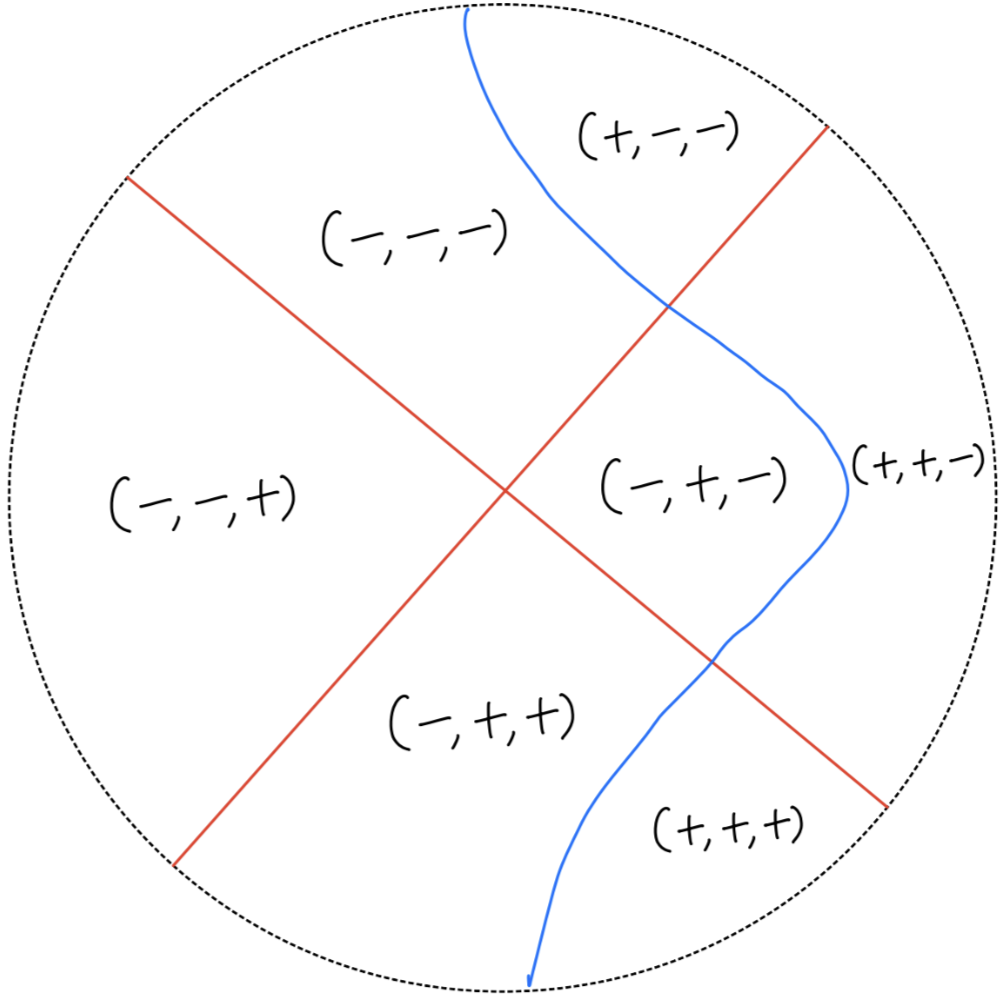
\includegraphics[scale = 0.45]{diagrams/lemma4/7.png}
    \caption{}
    \label{fig:your-label}
\end{figure}
\begin{figure}[H]
    \centering
    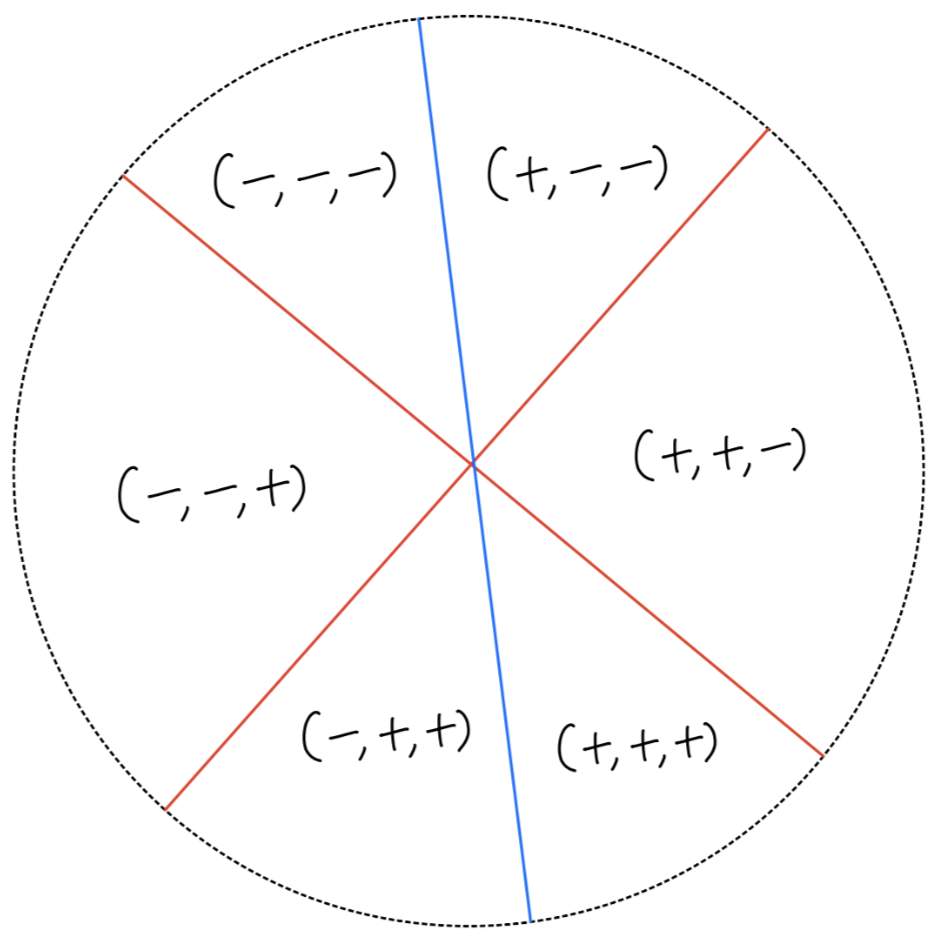
\includegraphics[scale = 0.45]{diagrams/lemma4/8.png}
    \caption{}
    \label{fig:your-label}
\end{figure}
\begin{figure}[H]
    \centering
    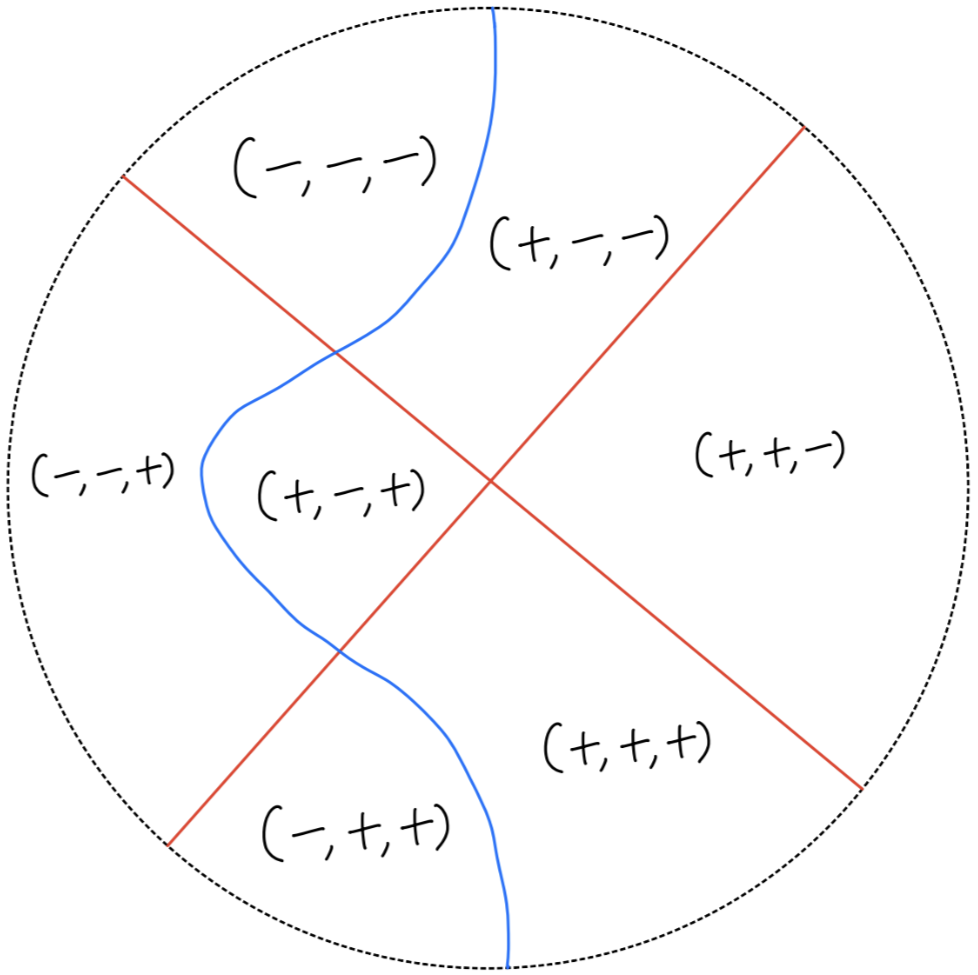
\includegraphics[scale = 0.45]{diagrams/lemma4/9.png}
    \caption{}
    \label{fig:your-label}
\end{figure}
\item $3$ dimensional strata: \\
$\{s_\bullet(sgn_2,sgn_1,sgn_3) ~|~ sgn_i \in \{-,+\}\text{ for i=1,2,3}\}$

\begin{figure}[H]
    \centering
    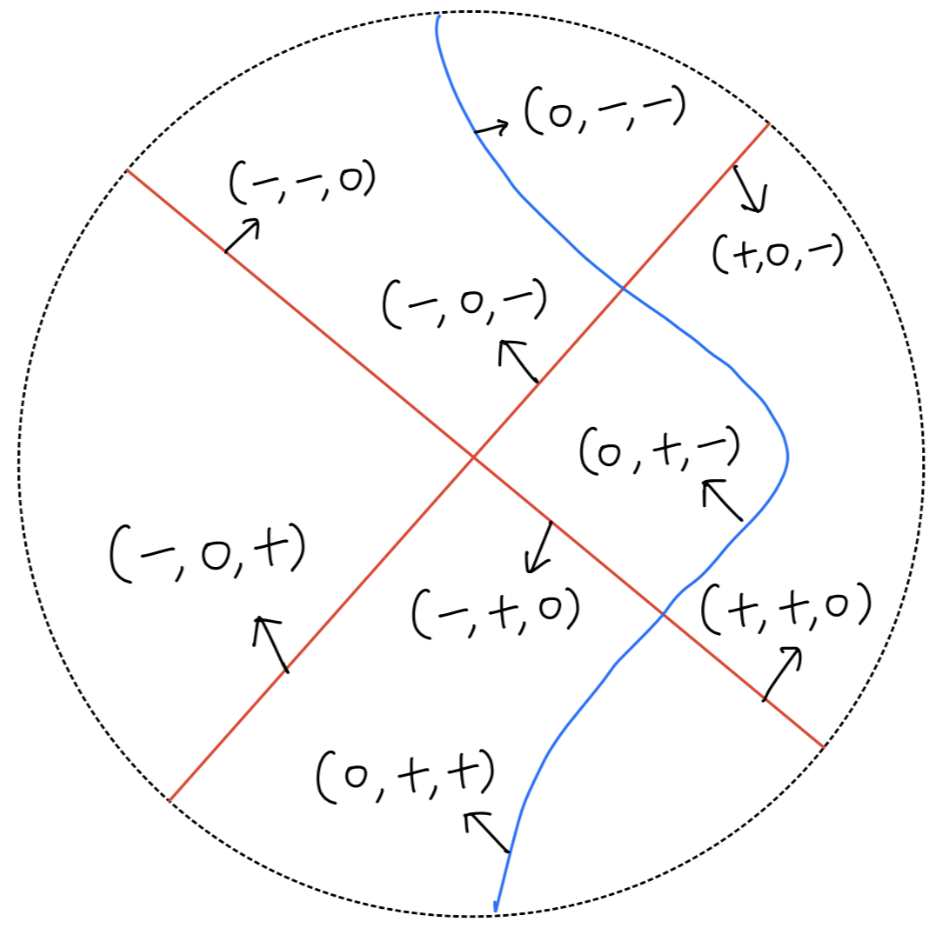
\includegraphics[scale = 0.45]{diagrams/lemma4/10.png}
    \caption{}
    \label{fig:your-label}
\end{figure}
\begin{figure}[H]
    \centering
    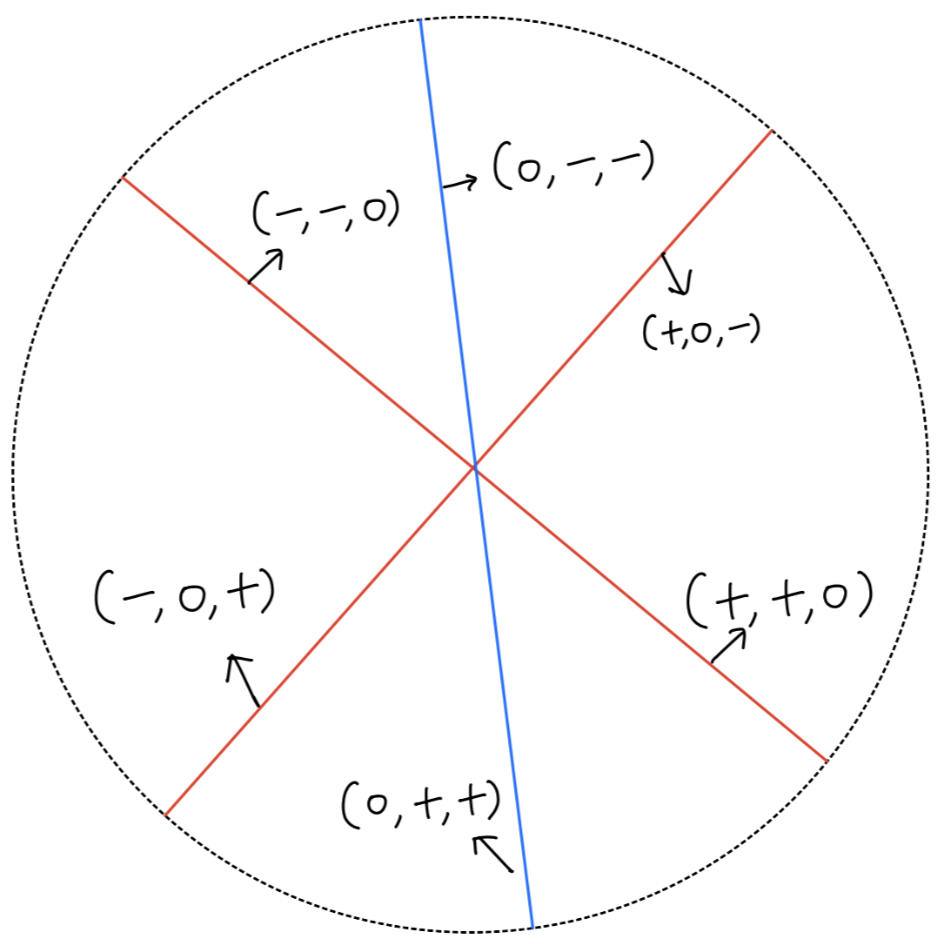
\includegraphics[scale = 0.45]{diagrams/lemma4/11.png}
    \caption{}
    \label{fig:your-label}
\end{figure}
\begin{figure}[H]
    \centering
    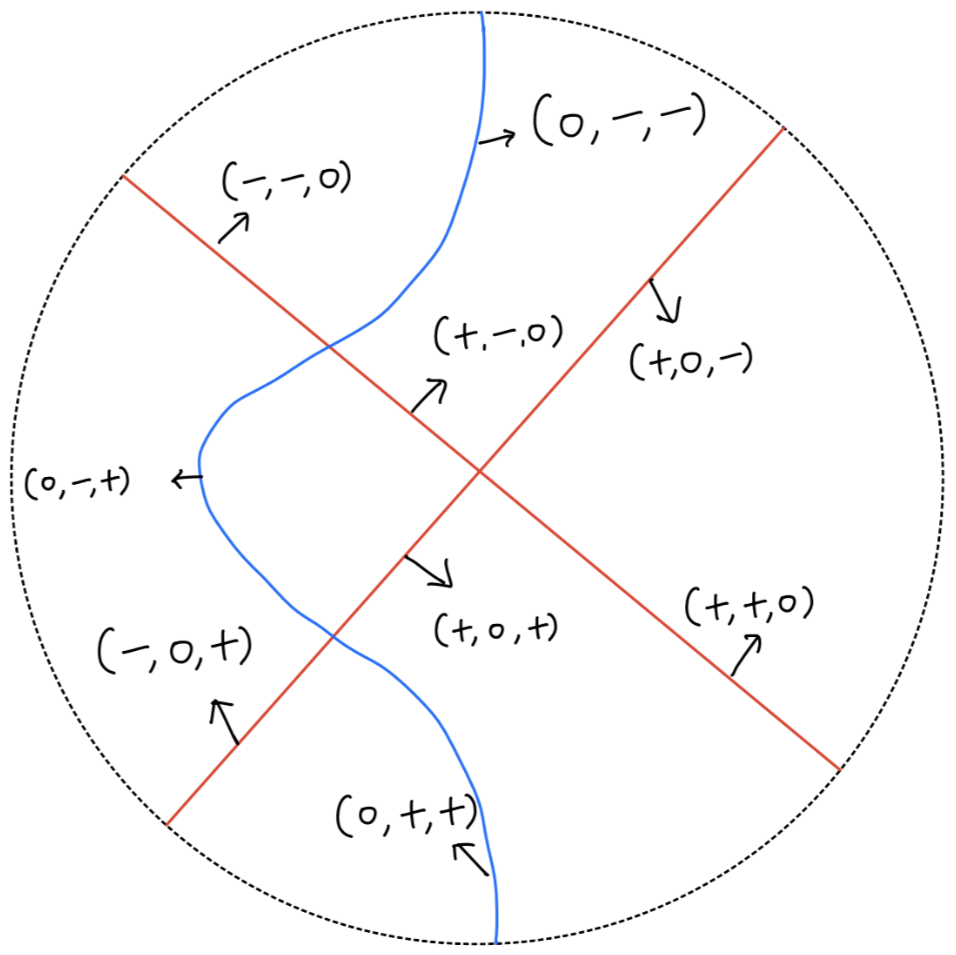
\includegraphics[scale = 0.45]{diagrams/lemma4/12.png}
    \caption{}
    \label{fig:your-label}
\end{figure}
\item $2$ dimensional strata: \\
$\{s_\bullet(0,sgn_2,sgn_3) ~|~ sgn_i \in \{-,+\}\text{ for i=2,3}\}\cup\{s_\bullet(sgn_1,0,sgn_3) ~|~ sgn_i \in \{-,+\}\text{ for i=1,3}\}\cup\{s_\bullet(sgn_1,sgn_2,0) ~|~ sgn_i \in \{-,+\}\text{ for i=1,2}\}$

\begin{figure}[H]
    \centering
    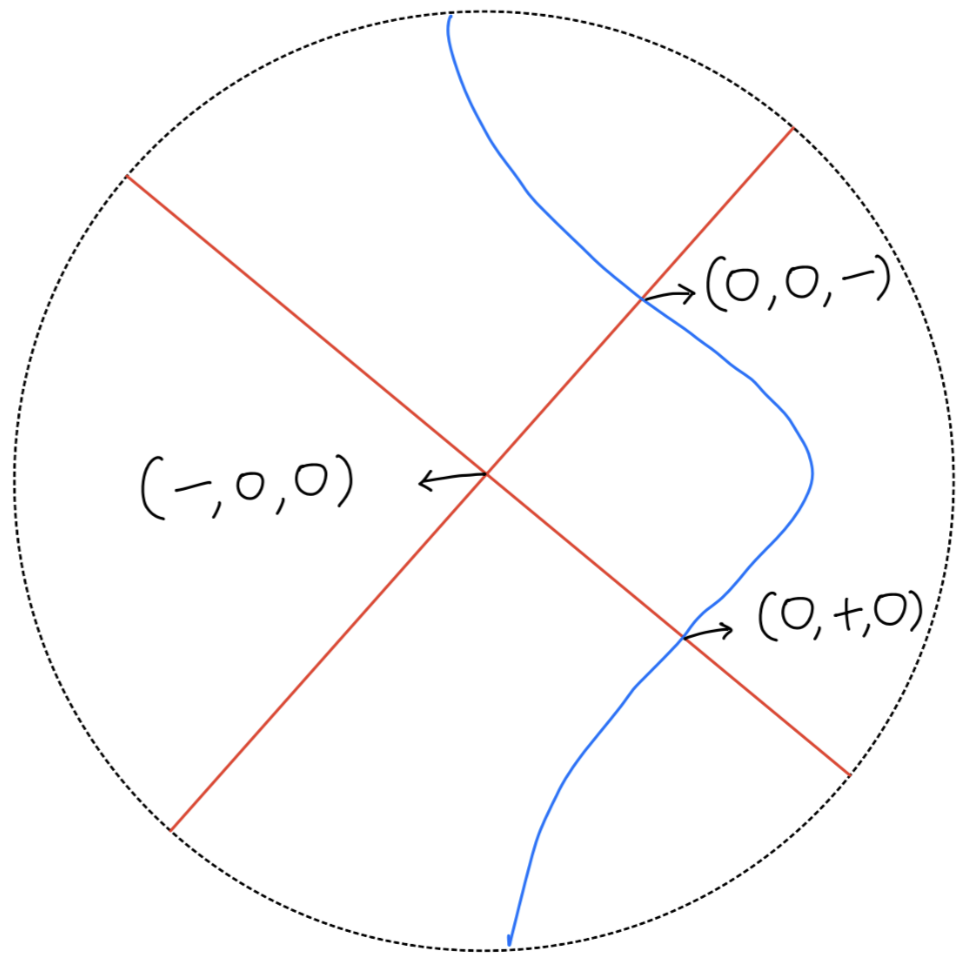
\includegraphics[scale = 0.45]{diagrams/lemma4/13.png}
    \caption{}
    \label{fig:your-label}
\end{figure}
\begin{figure}[H]
    \centering
    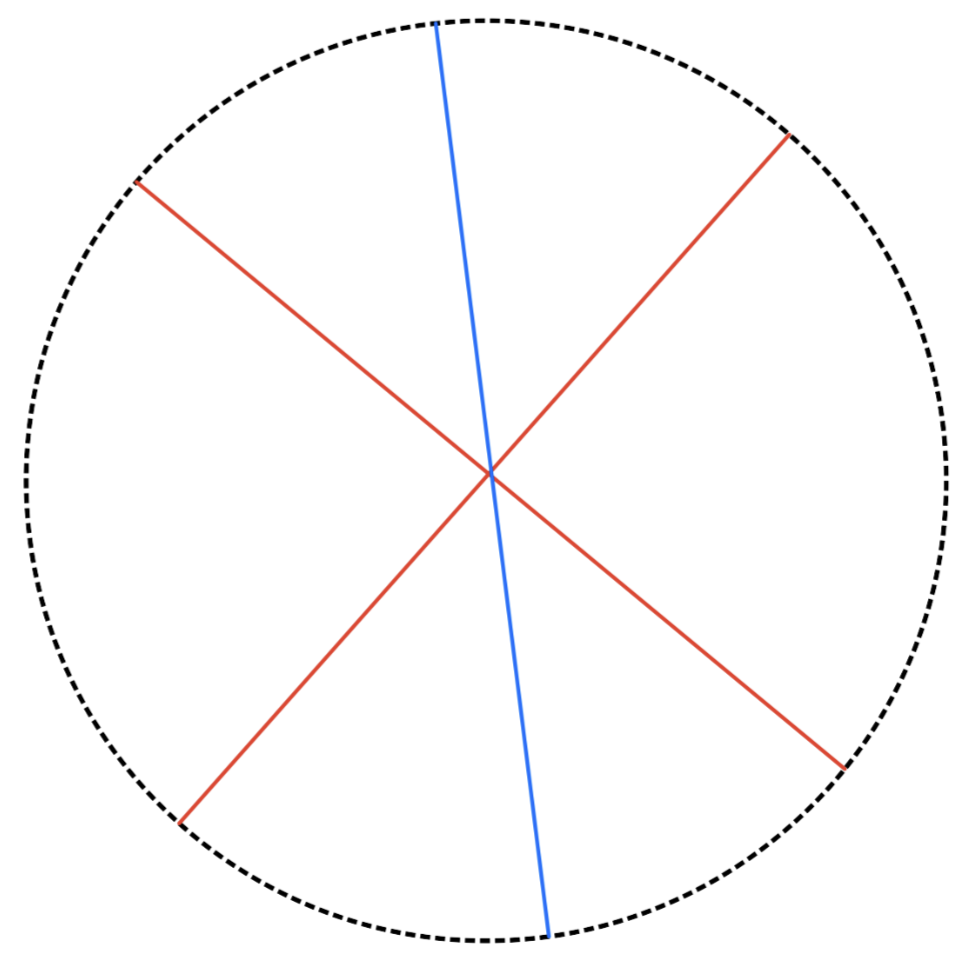
\includegraphics[scale = 0.45]{diagrams/lemma4/14.png}
    \caption{}
    \label{fig:your-label}
\end{figure}
\begin{figure}[H]
    \centering
    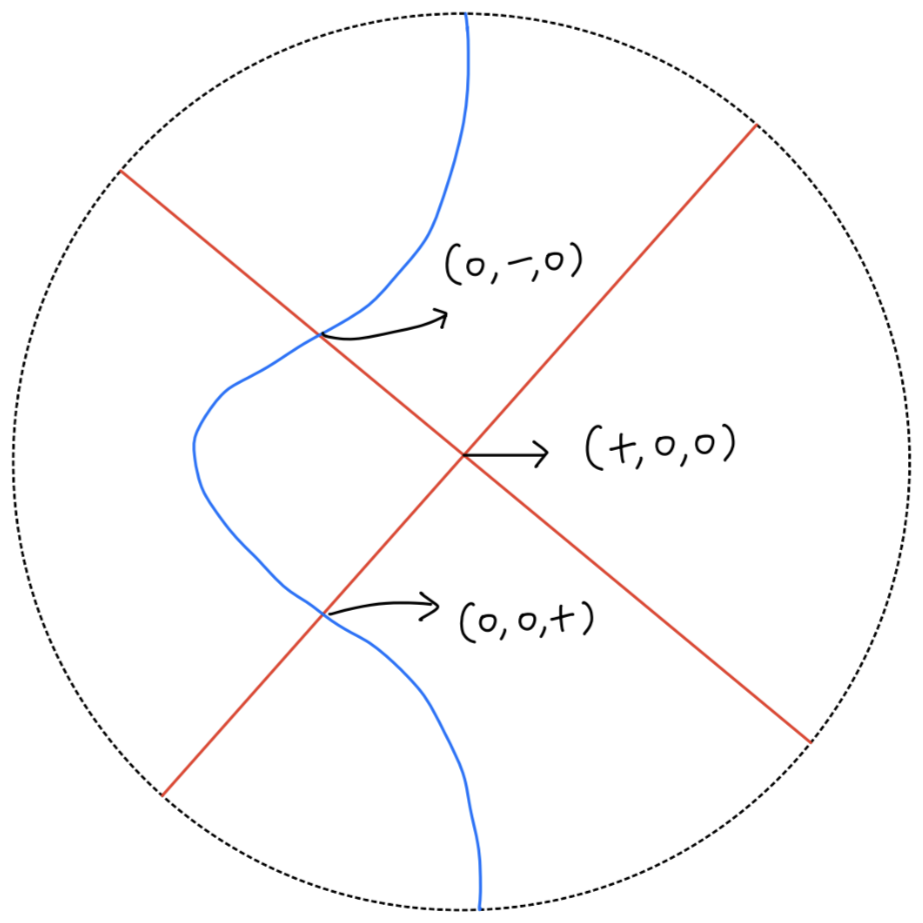
\includegraphics[scale = 0.45]{diagrams/lemma4/15.png}
    \caption{}
    \label{fig:your-label}
\end{figure}
\item $1$ dimensional strata: \\
$\{s_\bullet(sgn_1,0,0) ~|~ sgn_1 \in \{-,+\}\}\cup\{s_\bullet(0,sgn_2,0) ~|~ sgn_2 \in \{-,+\}\}\cup\{s_\bullet(0,0,sgn_3) ~|~ sgn_3 \in \{-,+\}\}$ 

\begin{figure}[H]
    \centering
    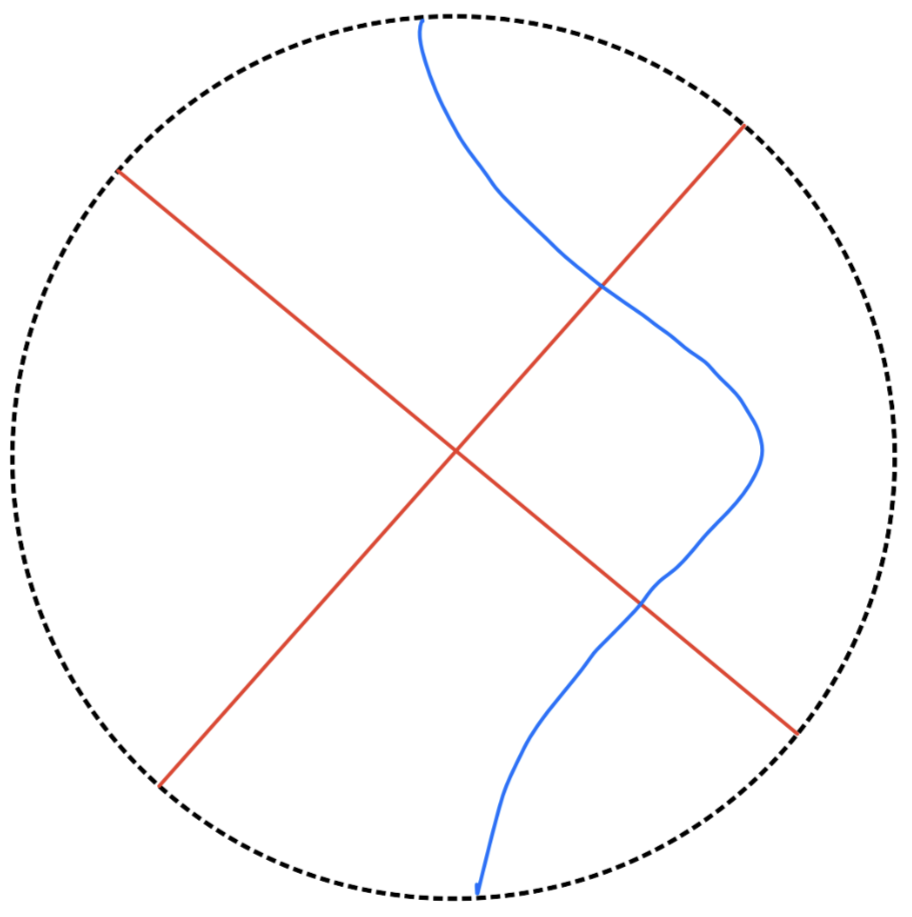
\includegraphics[scale = 0.45]{diagrams/lemma4/16.png}
    \caption{}
    \label{fig:your-label}
\end{figure}
\begin{figure}[H]
    \centering
    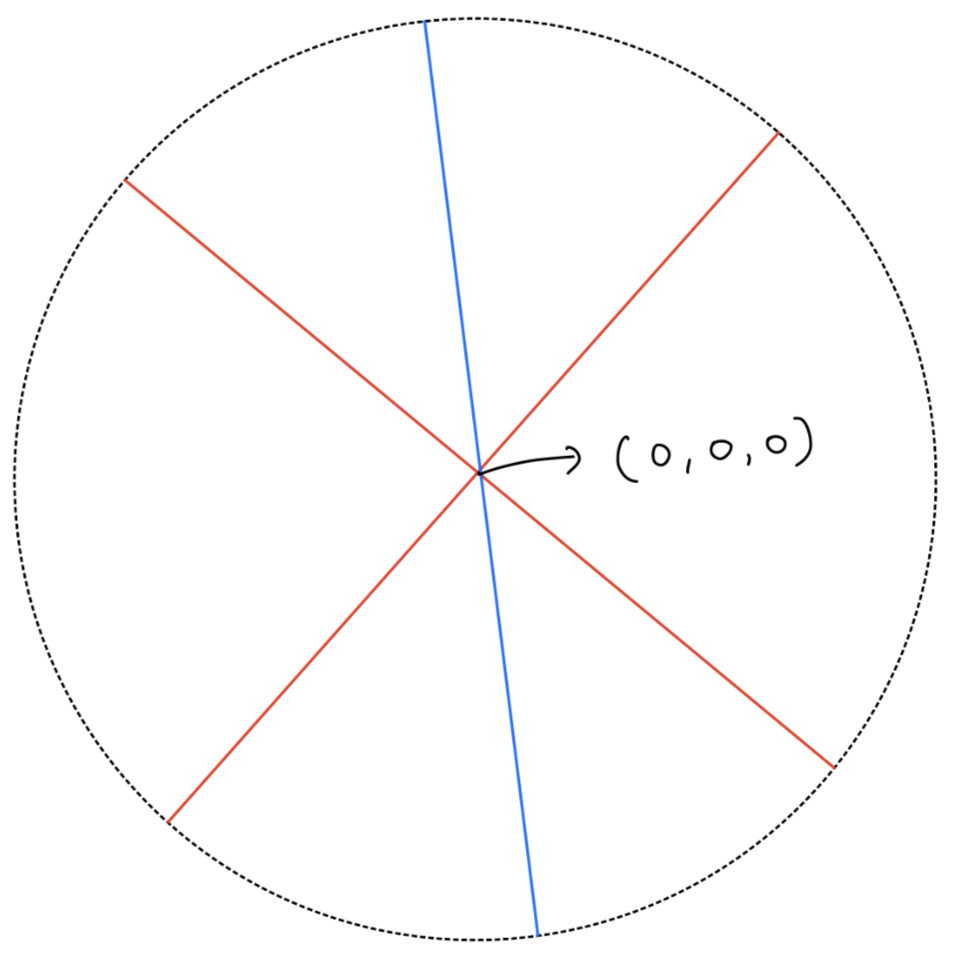
\includegraphics[scale = 0.45]{diagrams/lemma4/17.png}
    \caption{}
    \label{fig:your-label}
\end{figure}
\begin{figure}[H]
    \centering
    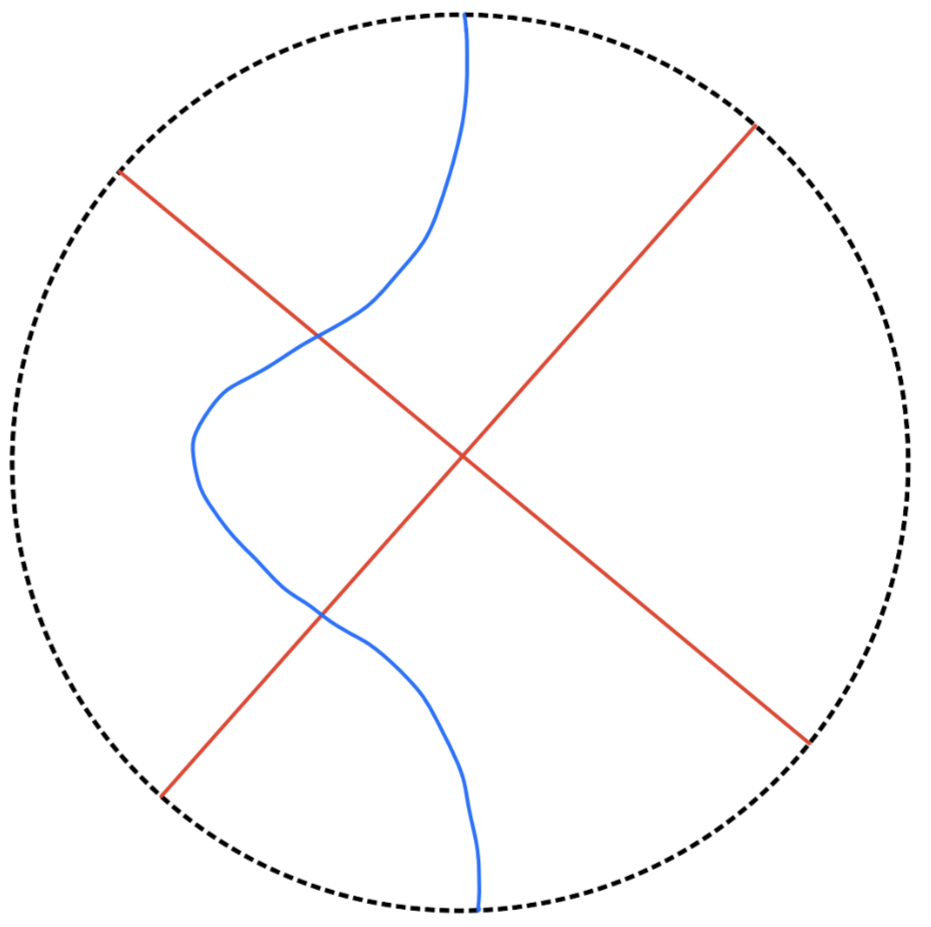
\includegraphics[scale = 0.45]{diagrams/lemma4/18.png}
    \caption{}
    \label{fig:your-label}
\end{figure}
\item $0$ dimensional strata: \\
$s_\bullet(0,0,0)$
\end{itemize}
\end{enumerate}
\end{definition}

% definition of the quiver associated to a squiggly diagram
\begin{definition}
Suppose we have a manifold $R$ with stratification $\mathcal{S}$ such that
\begin{itemize}
\item for each codimension $1$ stratum $s\in \mathcal{S}$, there are exactly two regions(= codimension $0$ strata) contained in $\operatorname{star}(s)$.

\item each codimension $1$ stratum is equipped with a co-orientation.
\end{itemize}
then we define the quiver associated to $\mathcal{S}$, say $Q_{\mathcal{S}}$, to be a quiver
\begin{itemize}
\item whose vertices corresponds to codimension $0$ strata of $\mathcal{S}$.

\item whose arrows corresponds to codimension $1$ strata of $\mathcal{S}$.

\item the source of an arrow corresponding to $s\in \mathcal{S}$ is  vertex corresponding to the region where the hairs of $s$ are pointing at and the target is the other region contained in the $\operatorname{star}(s)$.
\end{itemize}
\end{definition}

% definition of the subquiver associated to a stratum
\begin{definition}
Suppose we have a manifold $R$ with stratification $\mathcal{S}$ such that
\begin{itemize}
\item for each codimension $1$ stratum $s\in \mathcal{S}$, there are exactly two regions(= codimension $0$ strata) contained in $\operatorname{star}(s)$.

\item each codimension $1$ stratum is equipped with a co-orientation.
\end{itemize}
then for each $s\in \mathcal{S}$, we define the subquiver of $Q_{\mathcal{S}}$ associated to $s$, say $Q_{\mathcal{S},s}$, to be the full subquiver whose vertices are the ones that corresponds to the regions contained in the start of $s$.
\end{definition}

% definition of legible stratification, quiver
\begin{definition}
Suppose we have a manifold $R$ with stratification $\mathcal{S}$ such that
\begin{itemize}
\item for each codimension $1$ stratum $s\in \mathcal{S}$, there are exactly two regions(= codimension $0$ strata) contained in $\operatorname{star}(s)$.

\item each codimension $1$ stratum is equipped with a co-orientation.
\end{itemize}
then $\mathcal{S}$ is a legible stratification if for all $s\in\mathcal{S}$, $Q_{\mathcal{S},s}$ has the initial vertex. We say the quiver $Q_{\mathcal{S}}$ associated to $\mathcal{S}$ is legible if $\mathcal{S}$ is.
\end{definition}

% definition of legible representation
\begin{definition}
Suppose we have a manifold $R$ with stratification $\mathcal{S}$ such that
\begin{itemize}
\item for each codimension $1$ stratum $s\in \mathcal{S}$, there are exactly two regions(= codimension $0$ strata) contained in $\operatorname{star}(s)$.

\item each codimension $1$ stratum is equipped with a co-orientation.
\end{itemize}
then we say the quiver representation $F_{\mathcal{S}}$ of $Q_{\mathcal{S}}$ is a legible representation if
\begin{itemize}
\item $\mathcal{S}$ is legible.

\item for any $v,v' \in Vert(Q_{\mathcal{S}})$ and any paths $(a_1,a_2,\cdots,a_k)$,$(a'_1,a'_2,\cdots,a'_{k'})$ from $v$ to $v'$, $F_{\mathcal{S}}(a_k)\circ \cdots F_{\mathcal{S}}(a_1) = F_{\mathcal{S}}(a'_{k'})\circ \cdots F_{\mathcal{S}}(a'_1) $ i.e. the composition is path independent.
\end{itemize}
\end{definition}

% definition of \rho
\begin{definition}
Suppose we have a manifold $R$ with stratification $\mathcal{S}$ such that
\begin{itemize}
\item for each codimension $1$ stratum $s\in \mathcal{S}$, there are exactly two regions(= codimension $0$ strata) contained in $\operatorname{star}(s)$.

\item each codimension $1$ stratum is equipped with a co-orientation.
\end{itemize}
Supoose $\mathcal{S}$ is legible, then we define $\rho:\mathcal{S}\rightarrow \{s\in \mathcal{S} ~|~ \operatorname{codim}(s)=0 \}$ as
\[
\rho(s):=\text{the codimension $0$ stratum corresponding to the initial vertex of $Q_{\mathcal{S},s}$}
\]
\end{definition}

% definition of the sheaf associated to a legible diagram
\begin{definition}
Suppose we have a manifold $R$ with stratification $\mathcal{S}$ such that
\begin{itemize}
\item for each codimension $1$ stratum $s\in \mathcal{S}$, there are exactly two regions(= codimension $0$ strata) contained in $\operatorname{star}(s)$.

\item each codimension $1$ stratum is equipped with a co-orientation.
\end{itemize}
Suppose the quiver representation $F_\mathcal{S}$ of $Q_\mathcal{S}$ is legible, then we define the associated functor $\overline{F_\mathcal{S}}\in Obj(Fun(\mathcal{S}, \C))$ as follows:
\begin{itemize}
\item for $s\in \mathcal{S}$, $\overline{F_\mathcal{S}} := F_\mathcal{S}(\rho(s))$.

\item for $s_1,s_2 \in \mathcal{S}$ where $s_2 \subset \operatorname{star}(s_1)$, then $\overline{F_\mathcal{S}}(s_1 \rightarrow s_2)$ is defined as follows: choose a path from the vertex corresponding to $\rho(s_1)$ to $\rho(s_2)$ in $Q_\mathcal{S}$, say $(a_1,\cdots,a_k)$, then 
\[
\overline{F_\mathcal{S}}(s_1 \rightarrow s_2) := F_\mathcal{S}(a_k)\circ\cdots F_\mathcal{S}(a_1)
\] 
This is well-defined because $F_\mathcal{S}$ is legible.
\end{itemize}
\end{definition}

%%%%%%%%%%%%%%%%%%%%%%%%%%%%%%%%%%%%%%%%%%%%%%%%%%%%%%%%%%%%%%%%%%%
%%                            Setting                            %%
%%%%%%%%%%%%%%%%%%%%%%%%%%%%%%%%%%%%%%%%%%%%%%%%%%%%%%%%%%%%%%%%%%%
\subsection*{Setting}
Suppose on $M$, we have
\begin{itemize}
\item  a squiggly diagram $\Lambda_0$ on $M$

\item nested regions $U' \subset U \subset M$. Note that if we define $V:= M - \overline{U'}$, $\{U,V\}$ form an open cover of $M$.

\item a smooth chart from $D_{r=2}$, say $f: D  \rightarrow U \subset M$
\end{itemize}
such that 
\begin{itemize}
\item $D_{r=1}$ is mapped to $U'$ 

\item $\lambda_0^0$ is mapped to $\Lambda_0^0 |_{U}$

\item $\lambda_0^\infty$ is mapped to $\Lambda_0^\infty |_{U}$

\item $\lambda_0^{squig}$ is mapped to $\Lambda_0^{squig} |_{U}$
\end{itemize}

%%%%%%%%%%%%%%%%%%%%%%%%%%%%%%%%%%%%%%%%%%%%%%%%%%%%%%%%%%%%%%%%%%%
%%                         Initial Sheaf                         %%
%%%%%%%%%%%%%%%%%%%%%%%%%%%%%%%%%%%%%%%%%%%%%%%%%%%%%%%%%%%%%%%%%%%
\subsection*{Sheaf at the Beginning}
Suppose we have a sheaf $\mathscr{F}_0$ singular supported on $\Lambda_0$ such that $f^*\mathscr{F}_0$ is isomorphic to the sheaf described by the following squiggly legible diagram $F_0$.

For simplicity, we use the following notations
\[
F_0(sgn_1,sgn_2,sgn_3,sgn_4):= F_0(s_0(sgn_1,sgn_2,sgn_3,sgn_4))
\]

\textbf{Stalks:}
\begin{figure}[H]
    \centering
    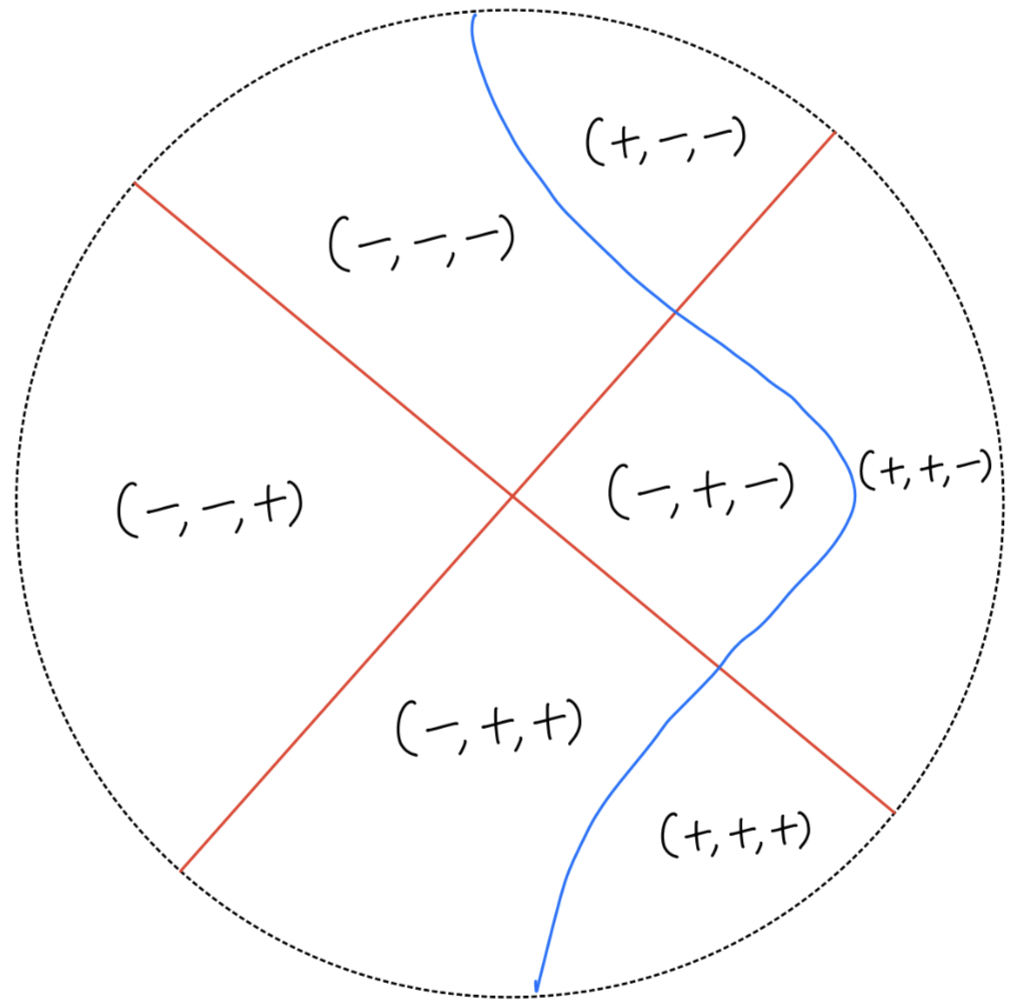
\includegraphics[scale = 0.45]{diagrams/lemma4/19.png}
    \caption{}
    \label{fig:your-label}
\end{figure}
\begin{figure}[H]
    \centering
    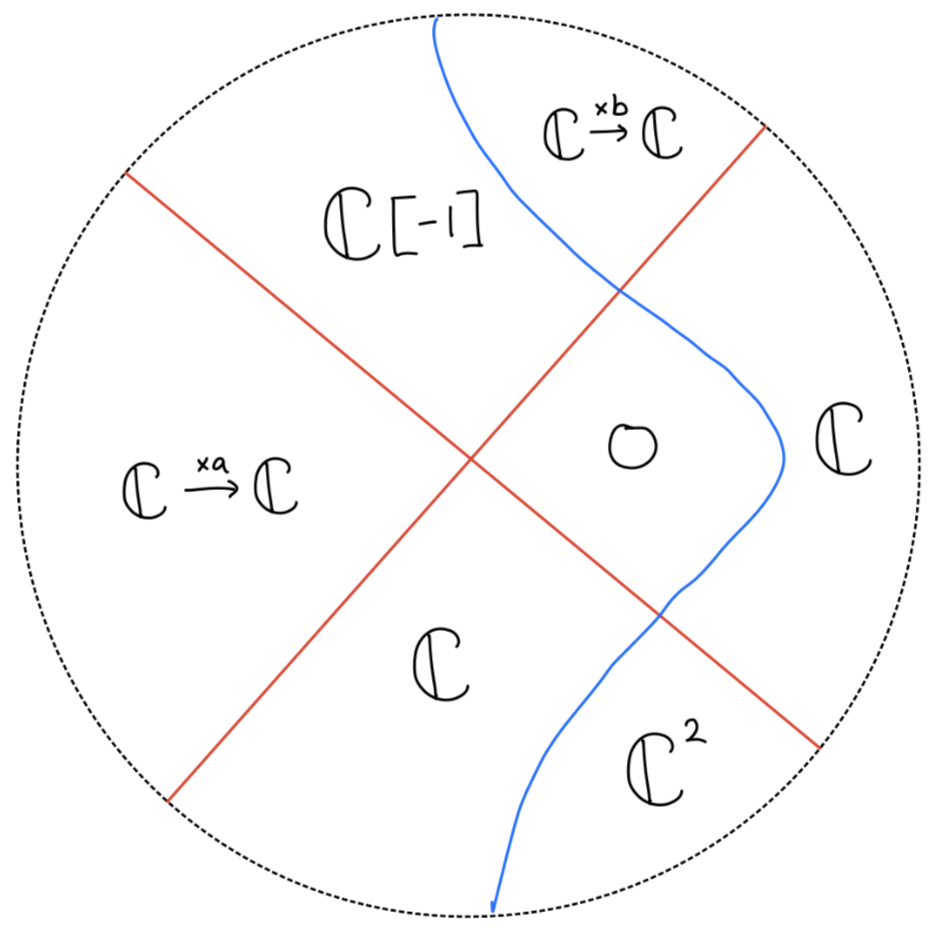
\includegraphics[scale = 0.45]{diagrams/lemma4/20.png}
    \caption{}
    \label{fig:your-label}
\end{figure}
\begin{itemize}
\item $F_0(-,-,-)$ := $\C[-1]$
\item $F_0(+,-,-)$ := $\C \xrightarrow{\times b} \C $
\item $F_0(-,-,+)$ := $\C \xrightarrow{\times a} \C $
\item $F_0(-,+,-)$ := $0$
\item $F_0(+,+,-)$ := $\C$
\item $F_0(-,+,+)$ := $\C$
\item $F_0(+,+,+)$ := $\C^2$
\end{itemize}
\textbf{Generization maps:}
\begin{figure}[H]
    \centering
    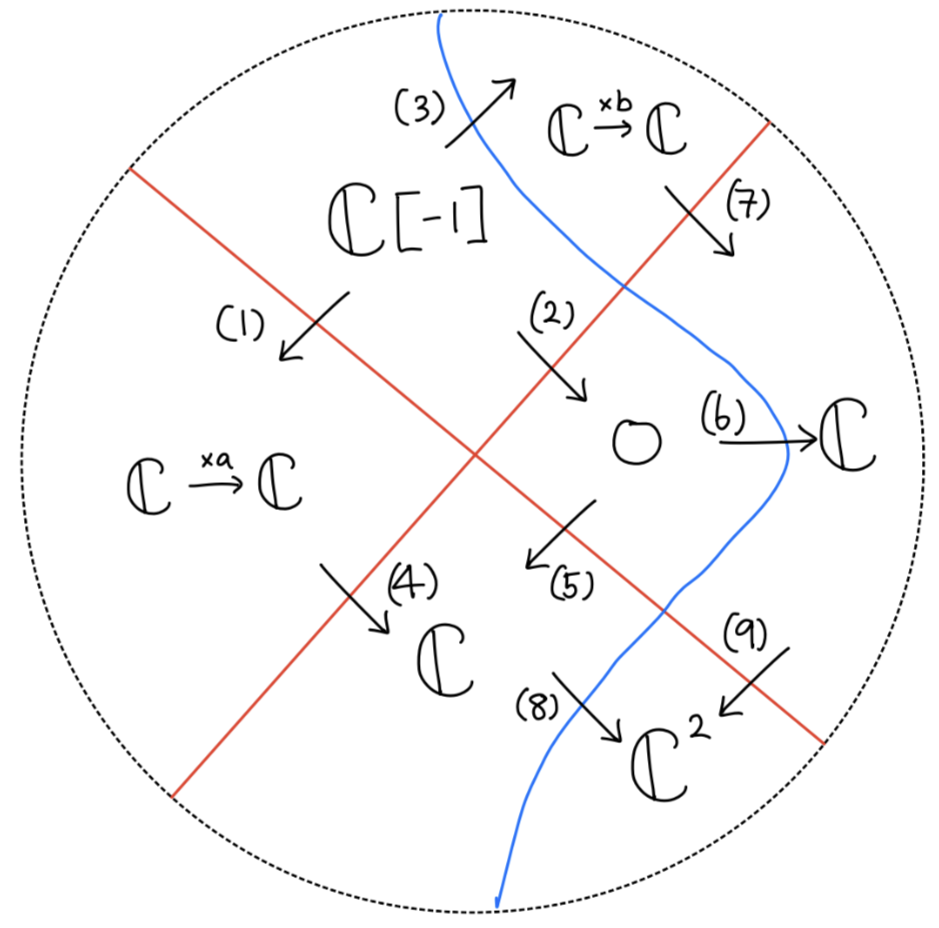
\includegraphics[scale = 0.45]{diagrams/lemma4/21.png}
    \caption{}
    \label{fig:your-label}
\end{figure}
\begin{enumerate}[label = (\arabic*)]
\item \begin{tikzcd}
\C \arrow[r, "\times 1"]     & \C  \\
0 \arrow[r]\arrow[u] & \C \arrow[u,"\times a"]
\end{tikzcd}

\item \begin{tikzcd}
\C \arrow[r]     & 0  \\
0 \arrow[r]\arrow[u] & 0 \arrow[u]
\end{tikzcd}

\item \begin{tikzcd}
\C \arrow[r, "\times 1"]     & \C  \\
0 \arrow[r]\arrow[u] & \C \arrow[u,"\times b"]
\end{tikzcd}

\item \begin{tikzcd}
\C \arrow[r]     & 0  \\
\C \arrow[r, "\times 1"]\arrow[u,"\times a"] & \C \arrow[u]
\end{tikzcd}

\item \begin{tikzcd}
0 \arrow[r]     & 0  \\
0 \arrow[r]\arrow[u] & \C \arrow[u]
\end{tikzcd}

\item \begin{tikzcd}
0 \arrow[r]     & 0  \\
0 \arrow[r]\arrow[u] & \C \arrow[u]
\end{tikzcd}

\item \begin{tikzcd}
\C \arrow[r]     & 0  \\
\C \arrow[r, "\times 1"]\arrow[u,"\times b"] & \C \arrow[u]
\end{tikzcd}

\item \begin{tikzcd}
0 \arrow[r]     & 0  \\
\C \arrow[r, "\iota_1"]\arrow[u] & \C^2 \arrow[u]
\end{tikzcd}

\item \begin{tikzcd}
0 \arrow[r]     & 0  \\
\C \arrow[r, "\iota_0"]\arrow[u] & \C^2 \arrow[u]
\end{tikzcd}

\end{enumerate}

%%%%%%%%%%%%%%%%%%%%%%%%%%%%%%%%%%%%%%%%%%%%%%%%%%%%%%%%%%%%%%%%%%%
%%                   Legendrian Cobordism                        %%
%%%%%%%%%%%%%%%%%%%%%%%%%%%%%%%%%%%%%%%%%%%%%%%%%%%%%%%%%%%%%%%%%%%
\subsection*{Legendrian Cobordism}
Then define a Legendrian cobordism $\mathscr{F}_\bullet$ starting from $\mathscr{F}_0$, say $cobord_4$, that is supported on $\overline{U'}$ as follows:\\

By Mayer-Vietoris, this equivalent to the following data
\begin{itemize}
\item a sheaf on $V\times [0,1]$, say $\mathscr{F}_{V\times [0,1]}$

\item a sheaf on $D_{r=2}\times [0,1]$, say $\mathscr{F}_{D_{r=2}\times [0,1]}$

\item a gluing isomorphsim, i.e. $\gamma_\bullet : (f_*\mathscr{F}_{D_{r=2}\times [0,1]})|_{(U\cap V)\times [0,1]} \xrightarrow{\sim} \mathscr{F}_{V\times [0,1]}|_{(U\cap V)\times [0,1]}$.
\end{itemize}
\subsubsection{A. Sheaf on $V\times [0,1]$}
First, I will define $\mathscr{F}_{V\times [0,1]}$ to be $pr_1^*(\mathscr{F}_0|_V)$ where $pr_1 : V \times [0,1] \rightarrow V$ is the projection onto the first argument.
\subsubsection{B. Sheaf on $D_{r=2}\times [0,1]$}
Next, I will describe $\mathscr{F}_{D_{r=2}\times [0,1]}$ as $F_\bullet \in Fun(\mathcal{S}_\bullet,\C)$ i.e. a functor from $\mathcal{S}_\bullet$ to the category of perfect $\C$-modules as follows: 

For simplicity, we use the following notations
\[
F_\bullet(sgn_1,sgn_2,sgn_3):= F_\bullet(s_\bullet(sgn_1,sgn_2,sgn_3))
\]

\textbf{Stalks:}
\begin{figure}[H]
    \centering
    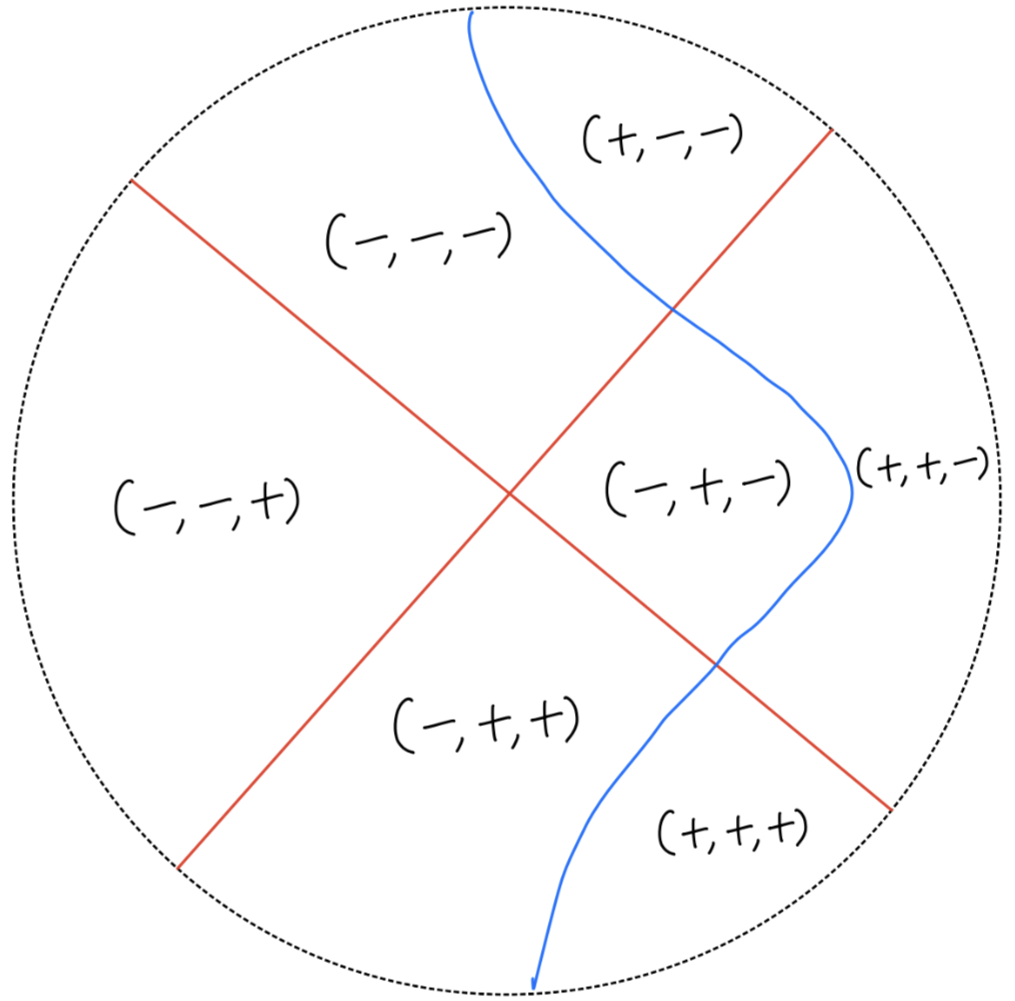
\includegraphics[scale = 0.45]{diagrams/lemma4/22.png}
    \caption{}
    \label{fig:your-label}
\end{figure}
\begin{figure}[H]
    \centering
    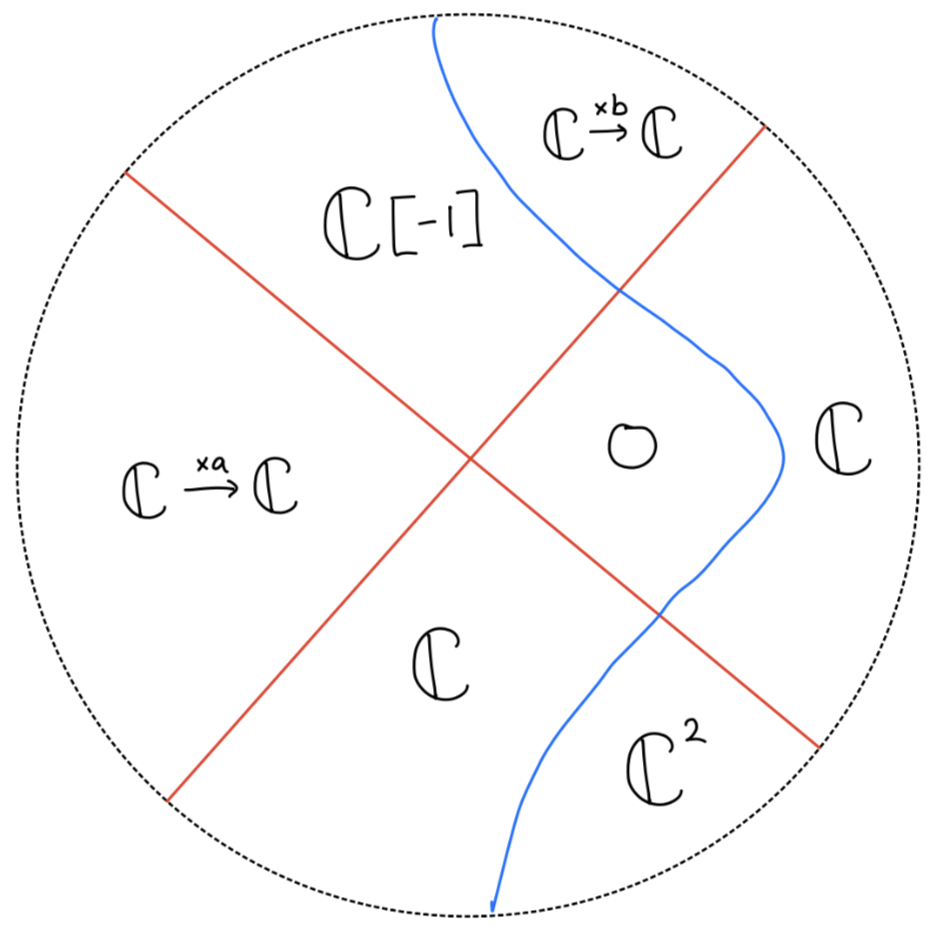
\includegraphics[scale = 0.45]{diagrams/lemma4/23.png}
    \caption{}
    \label{fig:your-label}
\end{figure}
\begin{figure}[H]
    \centering
    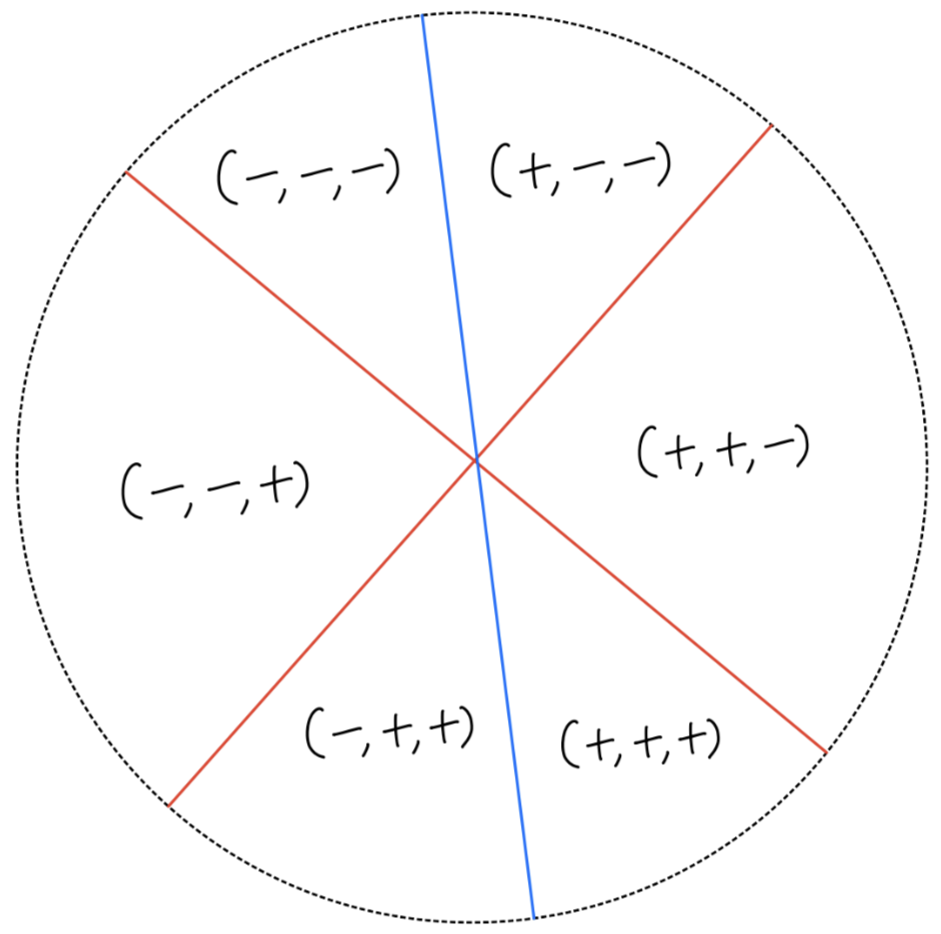
\includegraphics[scale = 0.45]{diagrams/lemma4/24.png}
    \caption{}
    \label{fig:your-label}
\end{figure}
\begin{figure}[H]
    \centering
    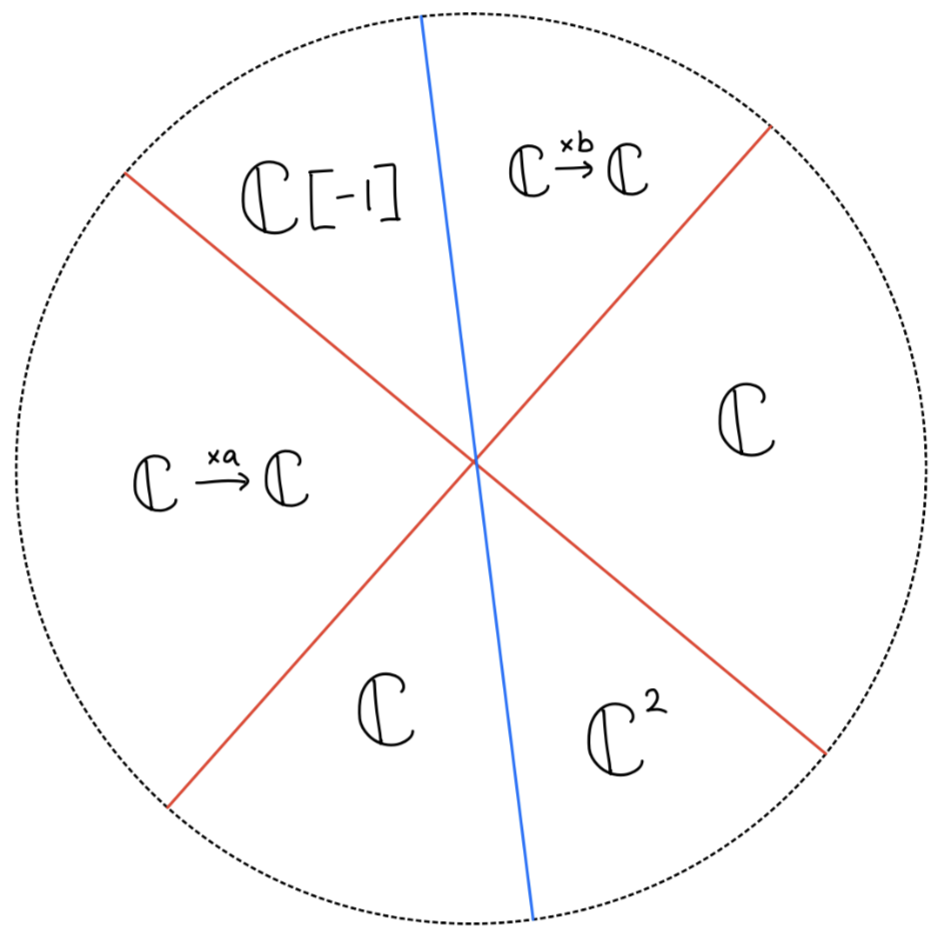
\includegraphics[scale = 0.45]{diagrams/lemma4/25.png}
    \caption{}
    \label{fig:your-label}
\end{figure}
\begin{figure}[H]
    \centering
    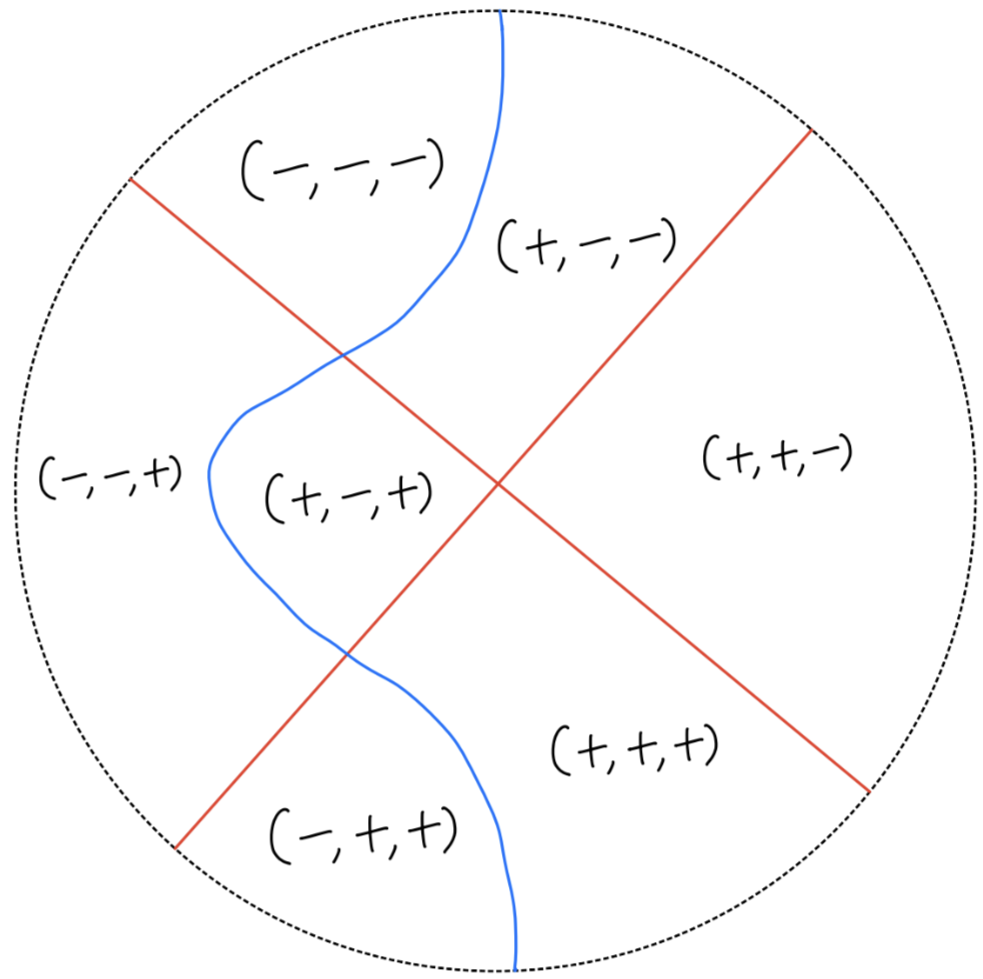
\includegraphics[scale = 0.45]{diagrams/lemma4/26.png}
    \caption{}
    \label{fig:your-label}
\end{figure}
\begin{figure}[H]
    \centering
    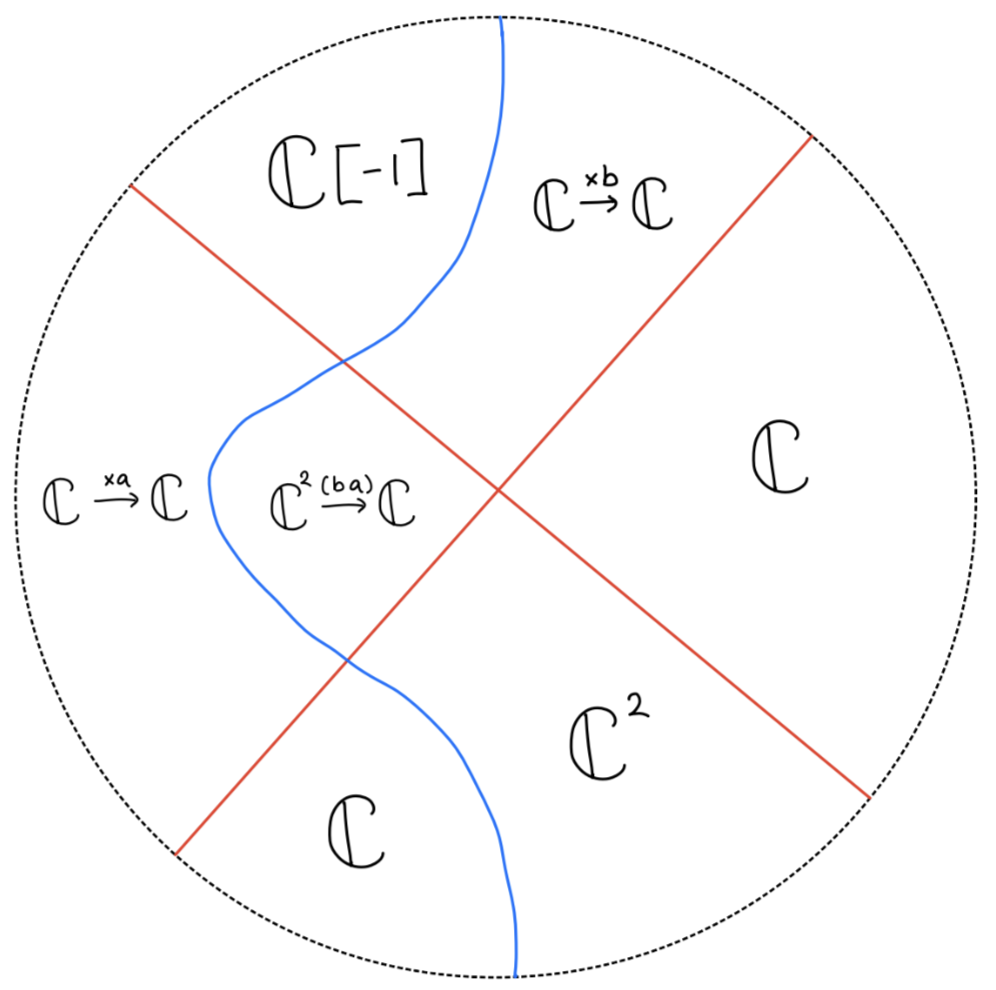
\includegraphics[scale = 0.45]{diagrams/lemma4/27.png}
    \caption{}
    \label{fig:your-label}
\end{figure}
\begin{itemize}
\item $F_\bullet(-,-,-)$ := $\C[-1]$
\item $F_\bullet(-,-,+)$ := $\C \xrightarrow{\times a} \C $
\item $F_\bullet(-,+,-)$ := $0$
\item $F_\bullet(-,+,+)$ := $\C$
\item $F_\bullet(+,-,-)$ := $\C \xrightarrow{\times b} \C $
\item $F_\bullet(+,-,+)$ := $\C^2 \xrightarrow{\times (b ~ a)} \C $
\item $F_\bullet(+,+,-)$ := $\C$
\item $F_\bullet(+,+,+)$ := $\C^2$
\end{itemize}

\textbf{Generization maps:}
\begin{figure}[H]
    \centering
    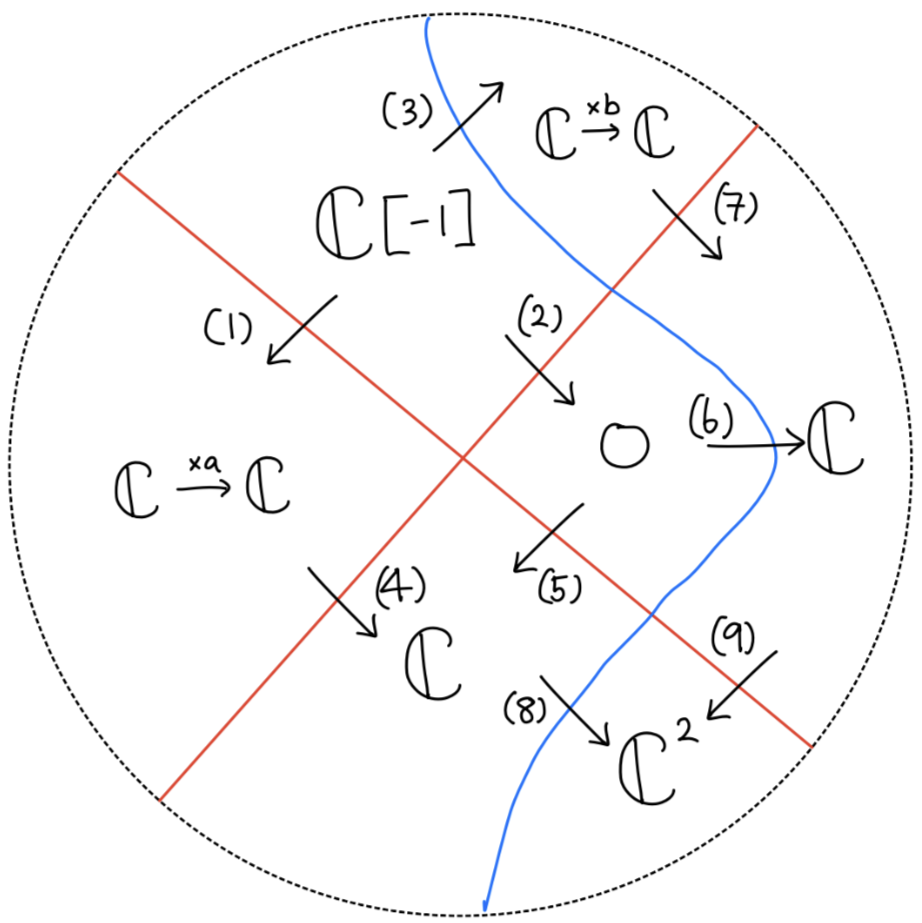
\includegraphics[scale = 0.45]{diagrams/lemma4/28.png}
    \caption{}
    \label{fig:your-label}
\end{figure}
\begin{figure}[H]
    \centering
    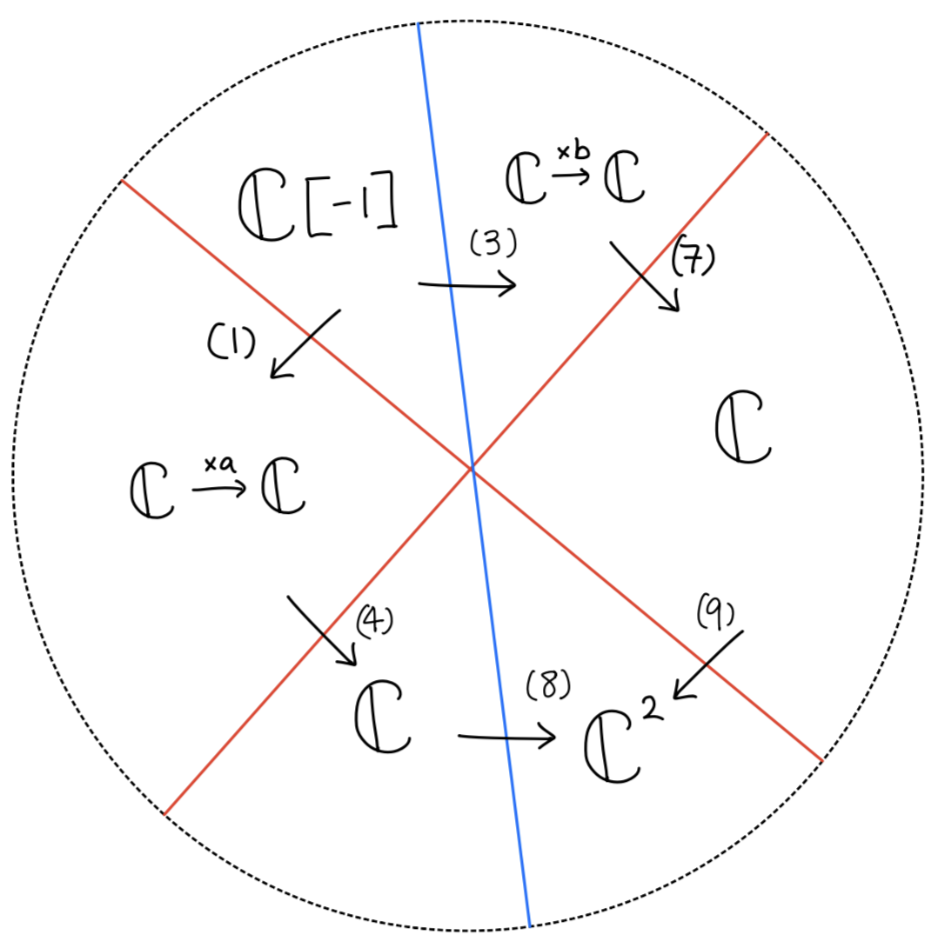
\includegraphics[scale = 0.45]{diagrams/lemma4/29.png}
    \caption{}
    \label{fig:your-label}
\end{figure}
Here!!!!!
\begin{figure}[H]
    \centering
    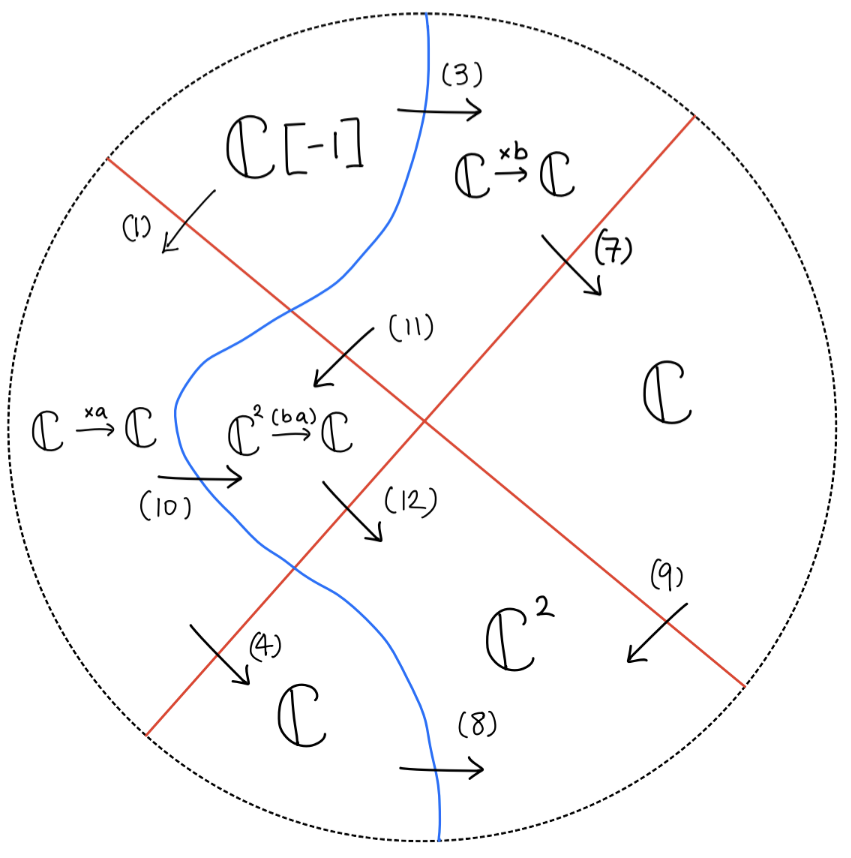
\includegraphics[scale = 0.45]{diagrams/lemma4/30.png}
    \caption{}
    \label{fig:your-label}
\end{figure}
\begin{enumerate}[label = (\arabic*)]
\item \begin{tikzcd}
\C \arrow[r, "\times 1"]     & \C  \\
0 \arrow[r]\arrow[u] & \C \arrow[u,"\times a"]
\end{tikzcd}

\item \begin{tikzcd}
\C \arrow[r]     & 0  \\
0 \arrow[r]\arrow[u] & 0 \arrow[u]
\end{tikzcd}

\item \begin{tikzcd}
\C \arrow[r, "\times 1"]     & \C  \\
0 \arrow[r]\arrow[u] & \C \arrow[u,"\times b"]
\end{tikzcd}

\item \begin{tikzcd}
\C \arrow[r]     & 0  \\
\C \arrow[r, "\times 1"]\arrow[u,"\times a"] & \C \arrow[u]
\end{tikzcd}

\item \begin{tikzcd}
0 \arrow[r]     & 0  \\
0 \arrow[r]\arrow[u] & \C \arrow[u]
\end{tikzcd}

\item \begin{tikzcd}
0 \arrow[r]     & 0  \\
0 \arrow[r]\arrow[u] & \C \arrow[u]
\end{tikzcd}

\item \begin{tikzcd}
\C \arrow[r]     & 0  \\
\C \arrow[r, "\times 1"]\arrow[u,"\times b"] & \C \arrow[u]
\end{tikzcd}

\item \begin{tikzcd}
0 \arrow[r]     & 0  \\
\C \arrow[r, "\iota_1"]\arrow[u] & \C^2 \arrow[u]
\end{tikzcd}

\item \begin{tikzcd}
0 \arrow[r]     & 0  \\
\C \arrow[r, "\iota_0"]\arrow[u] & \C^2 \arrow[u]
\end{tikzcd}

\item \begin{tikzcd}
\C \arrow[r, "\times 1"]     & \C  \\
\C \arrow[r, "\iota_1"]\arrow[u,"\times a"] & \C^2 \arrow[u, "(b ~ a)"]
\end{tikzcd}

\item \begin{tikzcd}
\C \arrow[r, "\times 1"]     & \C  \\
\C \arrow[r, "\iota_0"]\arrow[u,"\times b"] & \C^2 \arrow[u, "(b ~ a)"]
\end{tikzcd}

\item \begin{tikzcd}
\C \arrow[r]     & 0  \\
\C^2 \arrow[r, "id"]\arrow[u,"(b~a)"] & \C^2 \arrow[u]
\end{tikzcd}

\end{enumerate}

\subsubsection{C. Gluing Isomorphism}
Lastly, I will define a gluing isomorphism $\gamma_\bullet : (f_*\mathscr{F}_{D_{r=2}\times [0,1]})|_{(U\cap V)\times [0,1]} \xrightarrow{\sim} \mathscr{F}_{V\times [0,1]}|_{(U\cap V)\times [0,1]}$ using the fact that $(f_*\mathscr{F}_{D_{r=2}\times [0,1]})|_{(U\cap V)\times[0,1]}$ is isomorphic to $pr_1^*(\mathscr{F}_0|_{U\cap V})$ where $pr_1 : (U\cap V) \times [0,1] \rightarrow (U\cap V)$ is the projection onto the first argument.
\begin{definition}
we define $\gamma_\bullet$ to be the composition 
\[
(f_*\mathscr{F}_{D_{r=2}\times [0,1]})|_{(U\cap V)\times [0,1]}\xrightarrow{\sim}pr_1^*(\mathscr{F}_0|_{U\cap V})\xrightarrow{\sim}pr_1^*(\mathscr{F}_0|_{V})|_{(U\cap V)\times [0,1]}=\mathscr{F}_{V\times [0,1]}|_{(U\cap V)\times [0,1]}
\]
where
\begin{itemize}
\item the first isomorphism is the one mentioned in the above proposition.

\item the second isomorphism from the fact that the following diagram commutes:
\[
\begin{tikzcd}
(U\cap V)\times [0,1] \arrow[hookrightarrow]{r}\arrow[d, "pr_1"]     & V\times [0,1] \arrow[d, "pr_1"] \\
(U\cap V) \arrow[hookrightarrow]{r} & V 
\end{tikzcd}
\]
\end{itemize}
\end{definition}

Now we have defined a cobordism $\mathscr{F}_\bullet$, we show that this is a Legendrian cobordism.
\begin{proposition}
$\mathscr{F}_\bullet$ is a Legendrian cobordism i.e. $\mathscr{F}_\bullet \in Sh_\Lambda(M,\C)$.
\end{proposition}
\begin{proof}
To prove the claim, I will show that the microlocal stalks of $\mathscr{F}_\bullet$ vanishes at every points on a contangent bundle of $M$.\\
Note that there is a diffeomorphism beteween $D_{r=2} \times (0,1)$ and $\R^3$ that preserves there stratification i.e.
\[
s^3(sgn_1,sgn_2,sgn_3) \mapsto s_\bullet(sgn_1,sgn_2,sgn_3)
\]
Then it is enough to prove that the microlocal stalk of the pullback of $\mathscr{F}^\bullet$ along the above diffeomorphism vanishes at every points of $T^*\R^n$. The pullback of $\mathscr{F}^\bullet$ along the diffeomorphism could be described using the following legible diagram, say $F^3$. To simplify the notation, we denote
\[
F^3(sgn_1,sgn_2,sgn_3):= F^3(s^3(sgn_1,sgn_2,sgn_3))
\]
\textbf{Stalks:}
\begin{itemize}
\item $F^3(-,-,-)$ := $\C[-1]$
\item $F^3(-,-,+)$ := $\C\xrightarrow{\times a} \C$
\item $F^3(+,-,-)$ := $\C\xrightarrow{\times b} \C$
\item $F^3(+,-,+)$ := $\C^2 \xrightarrow{(b ~ a)} \C$
\item $F^3(-,+,-)$ := $0$
\item $F^3(-,+,+)$ := $\C$
\item $F^3(+,+,-)$ := $\C$
\item $F^3(+,+,+)$ := $\C^{2}$
\end{itemize}

\textbf{Generization maps:}\\
\begin{tikzcd}[row sep=1.5cm, column sep=2cm]
& s(-,+,-)\arrow[dd,"{(7)}"] \arrow[rr,"{(6)}"] & & s(-,+,+) \arrow[dd,"{(12)}"]\\
s(-,-,-) \arrow[dd,"{(3)}"]\arrow[rr,"{(1)}"] \arrow[ur,"{(2)}"] & & s(-,-,+) \arrow[dd,"{(5)}"]\arrow[ur,"{(4)}"]& \\
& s(+,+,-) \arrow[rr,"{(10)}"] & & s(+,+,+)  \\
s(+,-,-) \arrow[rr,"{(8)}"] \arrow[ur,"{(9)}"] & & s(+,-,+) \arrow[ur,"{(11)}"] &
\end{tikzcd}
\begin{enumerate}[label = (\arabic*)]
\item 
\begin{tikzcd}
\C \arrow[r,"\times 1"] & \C \\
0 \arrow[u]\arrow[r] & \C\arrow[u,"\times a"]
\end{tikzcd}

\item 
\begin{tikzcd}
\C \arrow[r,"\times a"] & 0 \\
0 \arrow[u]\arrow[r] & 0 \arrow[u]
\end{tikzcd}

\item 
\begin{tikzcd}
\C \arrow[r,"\times 1"] & \C \\
0 \arrow[u]\arrow[r] & \C\arrow[u,"\times b"]
\end{tikzcd}

\item 
\begin{tikzcd}
\C \arrow[r] & 0 \\
\C \arrow[u,"\times a"]\arrow[r,"\times 1"] & \C\arrow[u,]
\end{tikzcd}

\item 
\begin{tikzcd}
\C \arrow[r,"\times 1"] & \C \\
\C \arrow[u,"\times a"]\arrow[r,"\iota_1"] & \C^2\arrow[u,"(b~a)"]
\end{tikzcd}

\item 
\begin{tikzcd}
0 \arrow[r] & 0 \\
0 \arrow[u,]\arrow[r] & \C\arrow[u,]
\end{tikzcd}

\item 
\begin{tikzcd}
0 \arrow[r] & 0 \\
0 \arrow[u,]\arrow[r] & \C\arrow[u,]
\end{tikzcd}

\item 
\begin{tikzcd}
\C \arrow[r,"\times 1"] & \C \\
\C \arrow[u,"\times b"]\arrow[r,"\iota_0"] & \C^2\arrow[u,"(b~a)"]
\end{tikzcd}

\item 
\begin{tikzcd}
\C \arrow[r] & 0 \\
\C \arrow[u, "\times b"]\arrow[r, "\times 1"] & \C\arrow[u,]
\end{tikzcd}

\item 
\begin{tikzcd}
0 \arrow[r,] & 0 \\
\C \arrow[u,]\arrow[r,"\iota_0"] & \C^2\arrow[u,]
\end{tikzcd}

\item 
\begin{tikzcd}
\C \arrow[r,] & 0 \\
\C^2 \arrow[u,"(b~a)"]\arrow[r,"id"] & \C^2\arrow[u,]
\end{tikzcd}

\item 
\begin{tikzcd}
0 \arrow[r,] & 0 \\
\C \arrow[u,]\arrow[r,"\iota_1"] & \C^2\arrow[u,]
\end{tikzcd}
\end{enumerate}
To prove that microlocal stalk vanishes everywhere, by Lemma \ref{morse}, it is enough to show that the total complexes of $F^3$ restricted to the following squares and cubes are acyclic

\begin{enumerate}[label = (\roman*)]
\item 
\begin{tikzcd}
F^3(-,-,-) \arrow[r]\arrow[d] & F^3(-,+,-) \arrow[d] \\
F^3(+,-,-) \arrow[r] & F^3(+,+,-)
\end{tikzcd}
=
\begin{tikzcd}
\C[-1] \arrow[r,]\arrow[d,] & 0 \arrow[d, ] \\
\C\xrightarrow{\times a}\C \arrow[r,] & \C
\end{tikzcd}


\item 
\begin{tikzcd}
F^3(-,-,+) \arrow[r]\arrow[d] & F^3(-,+,+) \arrow[d] \\
F^3(+,-,+) \arrow[r] & F^3(+,+,+)
\end{tikzcd}
=
\begin{tikzcd}
\C\xrightarrow{\times a}\C \arrow[r, "{(\times 1,\times 0)}"]\arrow[d, "{(\iota_1,\times 1)}"] & \C \arrow[d, "\iota_1"] \\
\C^{2}\xrightarrow{(b~a)}\C \arrow[r, "{(id,0)}"] & \C^{2}
\end{tikzcd}

\item 
\begin{tikzcd}
F^3(-,-,-) \arrow[r]\arrow[d] & F^3(-,-,+) \arrow[d] \\
F^3(+,-,-) \arrow[r] & F^3(+,-,+)
\end{tikzcd}
=
\begin{tikzcd}
\C[-1] \arrow[r,"{(\times 0, \times 1)}"] \arrow[d, "{( \times 0,\times 1)}"] & \C\xrightarrow{\times a}\C \arrow[d,"{(\iota_1,\times 1)}"] \\
\C\xrightarrow{\times b} \C \arrow[r, "{(\iota_0,\times 1)}"] & \C^2 \xrightarrow{(b~a)}\C
\end{tikzcd}

\item 
\begin{tikzcd}
F^3(-,+,-) \arrow[r]\arrow[d] & F^3(-,+,+) \arrow[d] \\
F^3(+,+,-) \arrow[r] & F^3(+,+,+)
\end{tikzcd}
=
\begin{tikzcd}
0 \arrow[r, "\iota_0"]\arrow[d, "\iota_1"] & \C \arrow[d, "\iota_1"] \\
\C \arrow[r, "\iota_0"] & \C^{2}
\end{tikzcd}

\item 
\begin{tikzcd}
F^3(-,-,-) \arrow[r]\arrow[d] & F^3(-,-,+) \arrow[d] \\
F^3(-,+,-) \arrow[r] & F^3(-,+,+)
\end{tikzcd}
=
\begin{tikzcd}
\C[-1] \arrow[r, "{(\times 0,\times 1)}"]\arrow[d, ] & \C\xrightarrow{\times a}\C \arrow[d, "{(\times 1,\times 0)}"] \\
0 \arrow[r,] & \C
\end{tikzcd}

\item 
\begin{tikzcd}
F^3(+,-,-) \arrow[r]\arrow[d] & F^3(+,-,+) \arrow[d] \\
F^3(+,+,-) \arrow[r] & F^3(+,+,+)
\end{tikzcd}
=
\begin{tikzcd}
\C\xrightarrow{\times b}\C \arrow[r, "{(\iota_0,\times 1)}"]\arrow[d, "{( \times 1,\times 0)}"] & \C^{2}\xrightarrow{(b~a)}\C \arrow[d, "{( id, \times 0)}"] \\
\C \arrow[r, "\iota_0"] & \C^{2}
\end{tikzcd}

\item the cubic diagram:\\
\begin{tikzcd}[row sep=1.5cm, column sep=2cm]
& s(-,+,-)\arrow[dd,"{s(0,+,-)}"] \arrow[rr,"{s(-,+,0)}"] & & s(-,+,+) \arrow[dd,"{s(0,+,+)}"]\\
s(-,-,-) \arrow[dd,"{s(0,-,-)}"]\arrow[rr,"{s(-,-,0)}"] \arrow[ur,"{s(-,0,-)}"] & & s(-,-,+) \arrow[dd,"{s(0,-,+)}"]\arrow[ur,"{s(-,0,+)}"]& \\
& s(+,+,-) \arrow[rr,"{s(+,+,0)}"] & & s(+,+,+)  \\
s(+,-,-) \arrow[rr,"{s(+,-,0)}"] \arrow[ur,"{s(+,0,-)}"] & & s(+,-,+) \arrow[ur,"{s(+,0,+)}"] &
\end{tikzcd}\\
=\\
\begin{tikzcd}[row sep=2cm, column sep=2.5cm]
& 0 \arrow[dd,"0"]\arrow[rr,"0"] & & \C \arrow[dd,"{\iota_1}"] \\
\C[-1] \arrow[dd,"{(\times 0,\times 1)}"']\arrow[rr,"{(\times 0,\times 1)}"] \arrow[ur,"0"] & & \C\xrightarrow{\times a}\C \arrow[dd,"{( \iota_1,\times 1)}"]\arrow[ur,"{(\times 1,\times 0)}"']& \\
& \C \arrow[rr,"\iota_0"] & & \C^{2}  \\
\C\xrightarrow{\times b}\C \arrow[rr,"{(\iota_0,\times 1)}"] \arrow[ur,"{(\times 1,\times 0)}"] & & \C^{2}\xrightarrow{(b~a)}\C \arrow[ur,"{(id, \times 0)}"] &
\end{tikzcd}
\\ whose total complex is 
\[
\operatorname{Tot}(
\begin{tikzcd}
\C\xrightarrow{\times b}\C \arrow[r,"{(M_1,\times 1)}"]& \C^3\xrightarrow{(0~b~a)}\C \arrow[r,"{(M_2,\times 0)}"] &\C^2\\
0\rightarrow\C \arrow[u, "{( \times 0,\times 1)}"]\arrow[r,"{(\times 0,\times 1)}"]& \C\xrightarrow{\times a}\C \arrow[u,"{( M_3,\times 1)}"]\arrow[r, "{(\times (-1),\times 0)}"] &\C\arrow[u, "\iota_1"]\\
\end{tikzcd}
)
\]
where 
\begin{align*}
M_1 &=
\begin{pmatrix}
 1\\
 1\\
 0
\end{pmatrix}
\\
M_2 &= 
\begin{pmatrix} 
1 & -1 & 0\\ 
0 & 0 & -1 
\end{pmatrix}\\
M_3 &= 
\begin{pmatrix} 
0 \\ 
0 \\ 
1 
\end{pmatrix}
\end{align*}
\\ This is equal to
\[
\operatorname{Tot}(
\begin{tikzcd}
\C \arrow[r,"M_1"]& \C^2 \arrow[r,"M_2"] &\C \arrow[r] & 0\\
0 \arrow[u]\arrow[r]& \C^2 \arrow[u,"M_3"]\arrow[r, "M_5"] &\C\arrow[u, "M_4"]\arrow[r, "M_6"] & \C^2 \arrow[u]\\
\end{tikzcd}
)
\]

\begin{align*}
M_1 &=
\begin{pmatrix}
 1\\
 1
\end{pmatrix}
\\
M_2 &= 
\begin{pmatrix} 
1 & -1
\end{pmatrix}
\\
M_3 &= 
\begin{pmatrix} 
b & 0 \\ 
0 & a 
\end{pmatrix}
\\
M_4 &= 
\begin{pmatrix} 
0 & b & a & 0
\end{pmatrix}
\\
M_5 &= 
\begin{pmatrix} 
1 & 0 \\ 
1 & 0 \\
0 & -1 \\ 
0 & -1 
\end{pmatrix}
\\
M_6 &= 
\begin{pmatrix} 
1 & -1 & 0 & 0 \\ 
0 & 0 & -1 & 1
\end{pmatrix}
\end{align*}
which is the following cochain complex
\[
0 \rightarrow \C^3 \xrightarrow{M_1} \C^6 \xrightarrow{M_2} \C^3
\]
\begin{align*}
M_1 &= 
\begin{pmatrix} 
1 & -b & 0 \\
1 & 0 & -a \\ 
0 & 1 & 0 \\
0 & 1 & 0 \\
0 & 0 & -1 \\
0 & 0 & -1 
\end{pmatrix}
\\
M_2 &= 
\begin{pmatrix} 
1 & 1 & 0 & b & a & 0 \\ 
0 & 0 & 1 & -1 & 0 & 0 \\
0 & 0 & 0 & 0 & -1 & 1
\end{pmatrix}
\end{align*}
\\The final cochain complex is acyclic because of the following reasons
\begin{itemize}
\item $M_2\circ M_1 =0$
\item $M_1$ is a monomorphism
\item $M_2$ is an epimorphism
\end{itemize} 
\end{enumerate}
\end{proof}

%%%%%%%%%%%%%%%%%%%%%%%%%%%%%%%%%%%%%%%%%%%%%%%%%%%%%%%%%%%%%%%%%%%
%%                       Terminal Sheaf                          %%
%%%%%%%%%%%%%%%%%%%%%%%%%%%%%%%%%%%%%%%%%%%%%%%%%%%%%%%%%%%%%%%%%%%
\subsection*{Sheaf at the End}
In this subsection, I will describe the sheaf $\mathscr{F}_1$ at the end of the $cobord_4$. By Mayer-Vietoris, $\mathscr{F}_1:= \mathscr{F}_\bullet|_{M\times\{1\}}$ on $M \cong M\times\{1\}$ is equivalent to the following data
\begin{itemize}
\item a sheaf on $V$, say $\mathscr{F}_{V}$

\item a sheaf on $D_{r=2}$, say $\mathscr{F}_{D_{r=2}}$

\item a gluing isomorphsim $\gamma_1 : f_*\mathscr{F}_{D_{r=2}}|_{U\cap V} \xrightarrow{\sim} \mathscr{F}_{V}|_{U\cap V}$.
\end{itemize}

\subsubsection{A. Sheaf on $V$}
First, a sheaf on $V\cong V\times\{1\}$ is the restriction of $\mathscr{F}_{V\times [0,1]}$ to $V\times \{1\}$, i.e. $\mathscr{F}_{V\times [0,1]}|_{V\times \{1\}}= pr_1^*(\mathscr{F}_0|_V)|_{V\times \{1\}} = \mathscr{F}_0|_V$.
\subsubsection{B. Sheaf on $D_{r=2}$}
Next, a sheaf on $D_{r=2}\cong D_{r=2}\times \{1\}$ is the restriction of $\mathscr{F}_{D_{r=2}\times [0,1]}$ to $D_{r=2}\times \{1\}$, i.e. $\mathscr{F}_{D_{r=2}\times [0,1]} |_{D_{r=2}\times \{1\}}$. I will describe it as a squiggly legible diagram $F_1$ which is the restriction of $F_\bullet$ defined in the previous section.

For simplicity, we use the following notations
\[
F_1(sgn_1,sgn_2,sgn_3):= F_1(s_1(sgn_1,sgn_2,sgn_3))
\]
\textbf{Stalks:}
\begin{figure}[H]
    \centering
    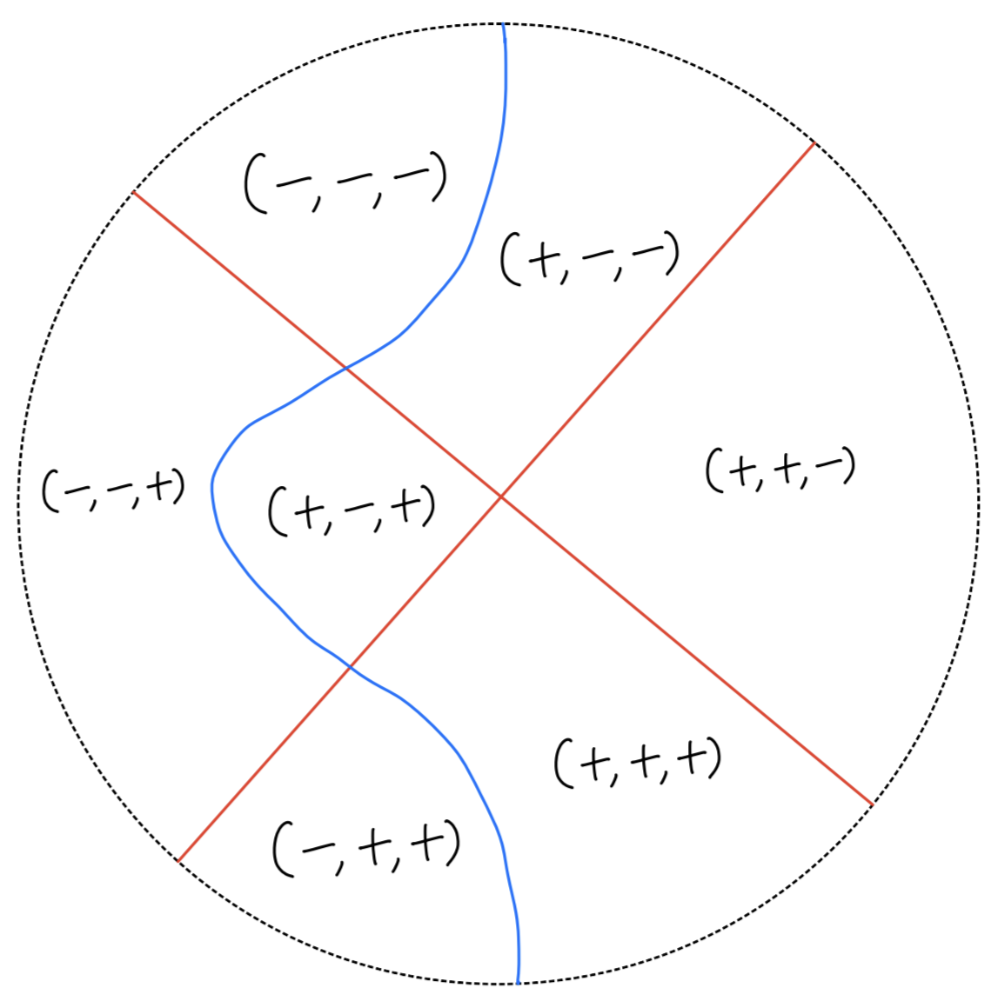
\includegraphics[scale = 0.45]{diagrams/lemma4/31.png}
    \caption{}
    \label{fig:your-label}
\end{figure}
\begin{figure}[H]
    \centering
    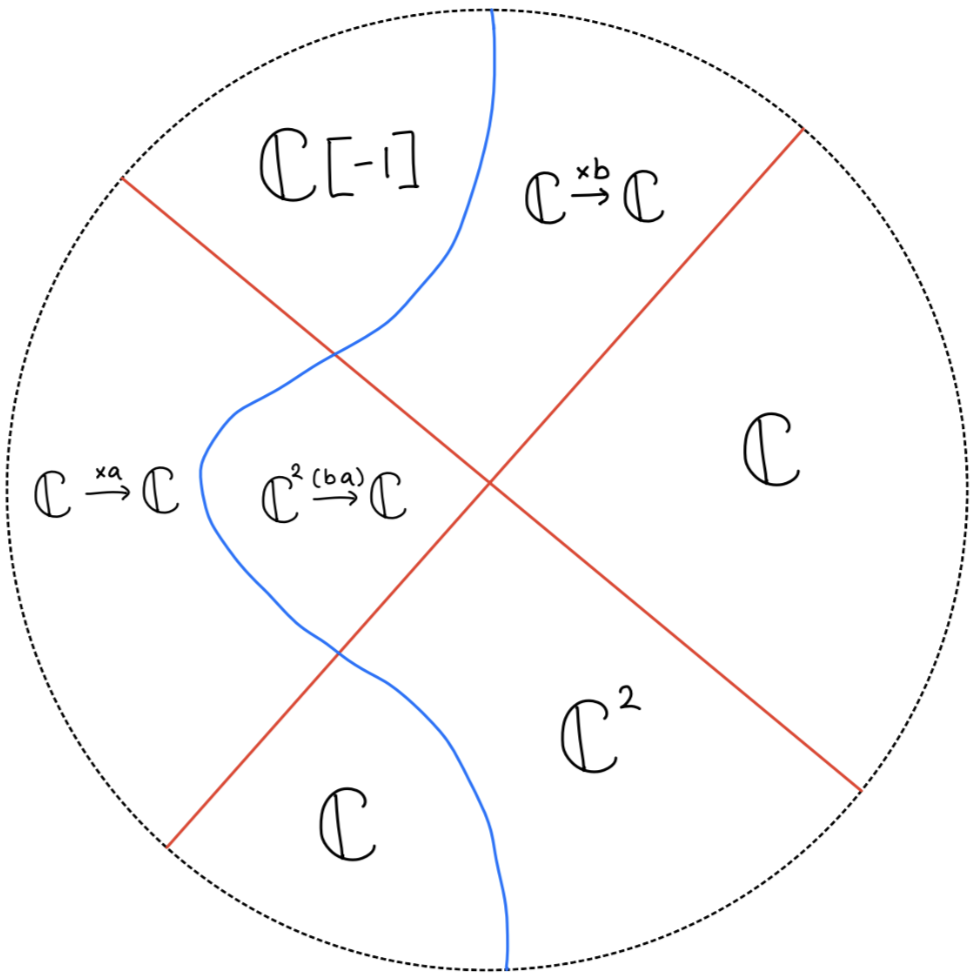
\includegraphics[scale = 0.45]{diagrams/lemma4/32.png}
    \caption{}
    \label{fig:your-label}
\end{figure}
\begin{itemize}
\item $F_1(-,-,-)$ := $\C[-1]$
\item $F_1(+,-,-)$ := $\C \xrightarrow{\times b} \C $
\item $F_1(-,-,+)$ := $\C \xrightarrow{\times a} \C $
\item $F_1(+,-,+)$ := $\C^2 \xrightarrow{(b ~ a)} \C $
\item $F_1(+,+,-)$ := $\C$
\item $F_1(-,+,+)$ := $\C$
\item $F_1(+,+,+)$ := $\C^2$
\end{itemize}
\textbf{Generization maps:}
\begin{figure}[H]
    \centering
    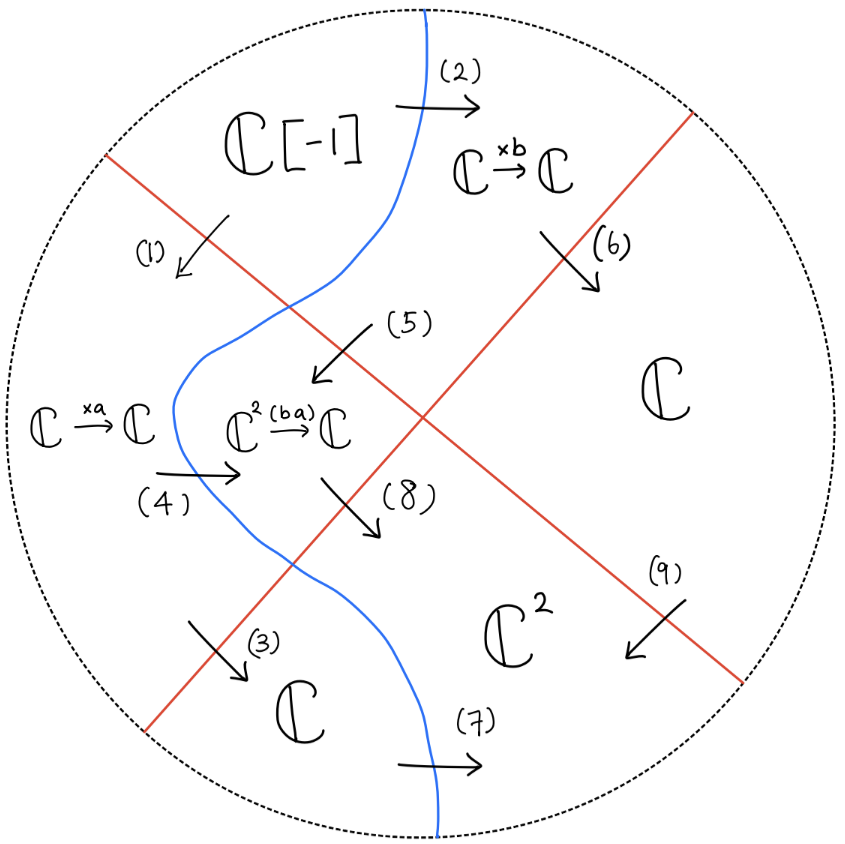
\includegraphics[scale = 0.45]{diagrams/lemma4/33.png}
    \caption{}
    \label{fig:your-label}
\end{figure}
\begin{enumerate}[label = (\arabic*)]
\item \begin{tikzcd}
\C \arrow[r, "\times 1"]     & \C  \\
0 \arrow[r]\arrow[u] & \C \arrow[u,"\times a"]
\end{tikzcd}

\item \begin{tikzcd}
\C \arrow[r, "\times 1"]     & \C  \\
0 \arrow[r]\arrow[u] & \C \arrow[u,"\times b"]
\end{tikzcd}

\item \begin{tikzcd}
\C \arrow[r]     & 0  \\
\C \arrow[r, "\times 1"]\arrow[u,"\times a"] & \C \arrow[u]
\end{tikzcd}

\item \begin{tikzcd}
\C \arrow[r, "\times 1"]     & \C  \\
\C \arrow[r, "\iota_1"]\arrow[u,"\times a"] & \C^2 \arrow[u, "(b ~ a)"]
\end{tikzcd}

\item \begin{tikzcd}
\C \arrow[r, "\times 1"]     & \C  \\
\C \arrow[r, "\iota_0"]\arrow[u,"\times b"] & \C^2 \arrow[u, "(b ~ a)"]
\end{tikzcd}

\item \begin{tikzcd}
\C \arrow[r]     & 0  \\
\C \arrow[r, "\times 1"]\arrow[u,"\times b"] & \C \arrow[u]
\end{tikzcd}

\item \begin{tikzcd}
0 \arrow[r]     & 0  \\
\C \arrow[r, "\iota_1"]\arrow[u] & \C^2 \arrow[u]
\end{tikzcd}

\item \begin{tikzcd}
\C \arrow[r]     & 0  \\
\C^2 \arrow[r, "id"]\arrow[u,"(b~a)"] & \C^2 \arrow[u]
\end{tikzcd}

\item \begin{tikzcd}
0 \arrow[r]     & 0  \\
\C \arrow[r, "\iota_0"]\arrow[u] & \C^2 \arrow[u]
\end{tikzcd}

\end{enumerate}

\subsubsection{C. Gluing Isomorphism}
Lastly, the gluing isomorphism $\gamma_1 := \gamma_\bullet|_{(U\cap V)\times \{1\}}:  f_*\mathscr{F}_{D_{r=2}}|_{(U\cap V)\times \{1\}}\xrightarrow{\sim} \mathscr{F}_0|_{U\cap V}$ is described as follows.

\begin{definition}
we define $\gamma_1$ to be the composition
\begin{align*}
&(f_*\mathscr{F}_{D_{r=2}})|_{(U\cap V)\times \{1\}}\xrightarrow{\sim}pr_1^*(\mathscr{F}_0|_{U\cap V})|_{(U\cap V)\times \{1\}}\xrightarrow{\sim}\mathscr{F}_0|_{U\cap V}
\end{align*}
where
\begin{itemize}
\item the first isomorphism follows from the fact that $(f_*\mathscr{F}_{D_{r=2}\times [0,1]})|_{(U\cap V)\times[0,1]}$ is isomorphic to $pr_1^*(\mathscr{F}_0|_{U\cap V})$.

\item the second isomorphism follows from the fact that the following composition is an identity map:
\[
(U\cap V)\xrightarrow{\sim} (U\cap V)\times \{1\} \hookrightarrow (U\cap V)\times [0,1] \twoheadrightarrow (U\cap V)
\]
\end{itemize}
\end{definition}
\pagebreak